\documentclass{article}

\usepackage{amsmath, amssymb, amsthm, enumerate}
\usepackage{blkarray}
\usepackage{tikz}
\usepackage{xcolor, soul}
\usepackage{tabularx}
\usetikzlibrary{cd}
\usetikzlibrary{matrix}
% \usepackage{url}

% theorems are included in the ACM version
\theoremstyle{definition}
\newtheorem{theorem}{Theorem}[section]
\newtheorem{corollary}[theorem]{Corollary}
\newtheorem{lemma}[theorem]{Lemma}
\newtheorem{proposition}[theorem]{Proposition}
\newtheorem{conjecture}[theorem]{Conjecture}
\newtheorem{definition}[theorem]{Definition}
\newtheorem{fact}[theorem]{Fact}
\newtheorem{example}[theorem]{Example}
\newtheorem{examples}[theorem]{Examples}
\newtheorem{example*}[theorem]{Example*}
\newtheorem{examples*}[theorem]{Examples*}
\newtheorem{remark}[theorem]{Remark}
\newtheorem{remark*}[theorem]{Remark*}
\newtheorem{question}[theorem]{Question}
\newtheorem{problem}[theorem]{Problem}
\newtheorem{assumption}[theorem]{Assumption}
\newtheorem{convention}[theorem]{Convention}

% begin Oxford stuff for diagrams
\usepackage{rotating}
\usepackage{floatpag}
\rotfloatpagestyle{empty}
\usepackage{hyperref}
\usepackage{xspace,color,epsfig}
\usepackage{graphicx}
\graphicspath{{.}{./figures/}}
\usepackage{marvosym}

\usepackage{tikzfig}
\usepackage{stmaryrd}
\usepackage{docmute}
\usepackage{keycommand}

\newcommand\nuclear{\omding\char195\xspace}
\newcommand\goodskull{\omding\char194\xspace}

\newcommand{\C}{\ensuremath{\mathbb{C}}}

\newcommand{\smallsum}{\textstyle{\sum\limits_i}}
\newcommand{\smallsumi}[1]{\textstyle{\sum\limits_{#1}}}

\newcommand{\emptydiag}{\,\tikz{\node[style=empty diagram] (x) {};}\,}
\newcommand{\scalar}[1]{\,\tikz{\node[style=scalar] (x) {$#1$};}\,}
\newcommand{\dscalar}[1]{\,\tikz{\node[style=scalar, doubled] (x) {$#1$};}\,}
\newcommand{\boxmap}[1]{\,\tikz{\node[style=small box] (x) {$#1$};\draw(0,-1)--(x)--(0,1);}\,}
\newcommand{\tboxmap}[3]{\,\begin{tikzpicture}
  \begin{pgfonlayer}{nodelayer}
    \node [style=small box] (0) at (0, 0) {$#1$};
    \node [style=none] (1) at (0, -0.5) {};
    \node [style=none] (2) at (0, -1.25) {};
    \node [style=none] (3) at (0, 1.25) {};
    \node [style=none] (4) at (0, 0.5) {};
    \node [style=right label] (5) at (0.25, -1) {$#2$};
    \node [style=right label] (6) at (0.25, 1) {$#3$};
  \end{pgfonlayer}
  \begin{pgfonlayer}{edgelayer}
    \draw (2.center) to (1.center);
    \draw (4.center) to (3.center);
  \end{pgfonlayer}
\end{tikzpicture}}
\newcommand{\boxstate}[1]{\,\tikz{\node[style=small box] (x) {$#1$};\draw(x)--(0,1);}\,}
\newcommand{\boxeffect}[1]{\,\tikz{\node[style=small box] (x) {$#1$};\draw(0,-1)--(x);}\,}
\newcommand{\boxmapTWOtoONE}[1]{\,\tikz{\node[style=small box] (x) {$#1$};\draw(-0.8,-1)--(x)--(0,1);\draw (0.8,-1)--(x);}\,}
\newcommand{\boxmapONEtoTWO}[1]{\,\tikz{\node[style=small box] (x) {$#1$};\draw(0,-1)--(x)--(-1,1);\draw (x)--(1,1);}\,}

\newcommand{\doubleop}{\ensuremath{\textsf{double}}\xspace}

\newcommand{\kscalar}[1]{\,\tikz{\node[style=kscalar] (x) {$#1$};}\,}
\newcommand{\kscalarconj}[1]{\,\tikz{\node[style=kscalarconj] (x) {$#1$};}\,}

\newcommand{\dmap}[1]{\,\tikz{\node[style=dmap] (x) {$#1$};\draw[boldedge] (0,-1.3)--(x)--(0,1.3);}\,}
\newcommand{\dmapdag}[1]{\,\tikz{\node[style=dmapdag] (x) {$#1$};\draw[boldedge] (0,-1.3)--(x)--(0,1.3);}\,}

\newcommand{\map}[1]{\,\tikz{\node[style=map] (x) {$#1$};\draw(0,-1.3)--(x)--(0,1.3);}\,}

\newcommand{\mapdag}[1]{\,\tikz{\node[style=mapdag] (x) {$#1$};\draw(0,-1.3)--(x)--(0,1.3);}\,}

\newcommand{\maptrans}[1]{\,\tikz{\node[style=maptrans] (x) {$#1$};\draw(0,-1.3)--(x)--(0,1.3);}\,}

\newcommand{\mapconj}[1]{\,\tikz{\node[style=mapconj] (x) {$#1$};\draw(0,-1.3)--(x)--(0,1.3);}\,}

\newcommand{\mapONEtoTWO}[1]{\,\begin{tikzpicture}
  \begin{pgfonlayer}{nodelayer}
    \node [style=map] (0) at (0, 0) {$#1$};
    \node [style=none] (1) at (0, -0.5) {};
    \node [style=none] (2) at (-0.75, 0.5) {};
    \node [style=none] (3) at (-0.75, 1.25) {};
    \node [style=none] (4) at (0, -1.25) {};
    \node [style=none] (5) at (0.75, 0.5) {};
    \node [style=none] (6) at (0.75, 1.25) {};
  \end{pgfonlayer}
  \begin{pgfonlayer}{edgelayer}
    \draw (4.center) to (1.center);
    \draw (2.center) to (3.center);
    \draw (5.center) to (6.center);
  \end{pgfonlayer}
\end{tikzpicture}\,}

\newkeycommand{\pointmap}[style=point][1]{\,\tikz{\node[style=\commandkey{style}] (x) at (0,-0.3) {$#1$};\node [style=none] (3) at (0, 1.0) {};\node [style=none] (3) at (0, -1.0) {};\draw (x)--(0,0.7);}\,}
\newcommand{\graypointmap}[1]{\pointmap[style=gray point]{#1}}

\newcommand{\dpointmap}[1]{\,\tikz{\node[style=point,doubled] (x) at (0,-0.3) {$#1$};\draw[boldedge] (x)--(0,0.7);}\,}
\newcommand{\dcopointmap}[1]{\,\tikz{\node[style=copoint, doubled] (x) at (0,0.3) {$#1$};\draw[boldedge] (x)--(0,-0.7);}\,}

\newcommand{\dpoint}[1]{\,\tikz{\node[style=point,doubled] (x) at (0,-0.3) {$#1$};\draw[boldedge] (x)--(0,0.7);}\,}
\newcommand{\dcopoint}[1]{\,\tikz{\node[style=copoint, doubled] (x) at (0,0.3) {$#1$};\draw[boldedge] (x)--(0,-0.7);}\,}

\newcommand{\kpoint}[1]{\,\tikz{\node[style=kpoint] (x) at (0,-0.05) {$#1$};\draw (x)--(0,0.9);}\,}
\newcommand{\kpointconj}[1]{\,\tikz{\node[style=kpoint conjugate] (x) at (0,-0.05) {$#1$};\draw (x)--(0,0.9);}\,}

\newcommand{\kpointdag}[1]{\,\tikz{\node[style=kpoint adjoint] (x) at (0,0.05) {$#1$};\draw (x)--(0,-0.9);}\,}
\newcommand{\kpointadj}[1]{\kpointdag{#1}}
\newcommand{\kpointtrans}[1]{\,\tikz{\node[style=kpoint transpose] (x) at (0,0.05) {$#1$};\draw (x)--(0,-0.9);}\,}

\newkeycommand{\typedkpoint}[style=kpoint,edgestyle=][2]{%
\,\begin{tikzpicture}
  \begin{pgfonlayer}{nodelayer}
    \node [style=none] (0) at (0, 1) {};
    \node [style=\commandkey{style}] (1) at (0, -0.75) {$#2$};
    \node [style=right label] (2) at (0.25, 0.5) {$#1$};
  \end{pgfonlayer}
  \begin{pgfonlayer}{edgelayer}
    \draw [\commandkey{edgestyle}] (1) to (0.center);
  \end{pgfonlayer}
\end{tikzpicture}\,}

\newkeycommand{\typedkpointdag}[style=kpoint adjoint,edgestyle=][2]{%
\,\begin{tikzpicture}
  \begin{pgfonlayer}{nodelayer}
    \node [style=none] (0) at (0, -1) {};
    \node [style=\commandkey{style}] (1) at (0, 0.75) {$#2$};
    \node [style=right label] (2) at (0.25, -0.5) {$#1$};
  \end{pgfonlayer}
  \begin{pgfonlayer}{edgelayer}
    \draw [\commandkey{edgestyle}] (0.center) to (1);
  \end{pgfonlayer}
\end{tikzpicture}\,}

\newcommand{\typedpoint}[2]{\,\begin{tikzpicture}
  \begin{pgfonlayer}{nodelayer}
    \node [style=none] (0) at (0, 1) {};
    \node [style=point] (1) at (0, -0.5) {$#2$};
    \node [style=right label] (2) at (0.25, 0.5) {$#1$};
  \end{pgfonlayer}
  \begin{pgfonlayer}{edgelayer}
    \draw (1) to (0.center);
  \end{pgfonlayer}
\end{tikzpicture}\,}

\newcommand{\bistate}[1]{\,\begin{tikzpicture}
  \begin{pgfonlayer}{nodelayer}
    \node [style=kpoint, minimum width=1 cm, inner sep=2pt] (0) at (0, -0.25) {$#1$};
    \node [style=none] (1) at (-0.75, 0) {};
    \node [style=none] (2) at (0.75, 0) {};
    \node [style=none] (3) at (-0.75, 0.75) {};
    \node [style=none] (4) at (0.75, 0.75) {};
  \end{pgfonlayer}
  \begin{pgfonlayer}{edgelayer}
    \draw (1.center) to (3.center);
    \draw (2.center) to (4.center);
  \end{pgfonlayer}
\end{tikzpicture}\,}

\newcommand{\bistateadj}[1]{\,\begin{tikzpicture}[yshift=-3mm]
  \begin{pgfonlayer}{nodelayer}
    \node [style=kpointadj, minimum width=1 cm, inner sep=2pt] (0) at (0, 0.5) {$\psi$};
    \node [style=none] (1) at (-0.75, 0.25) {};
    \node [style=none] (2) at (0.75, 0.25) {};
    \node [style=none] (3) at (-0.75, -0.5) {};
    \node [style=none] (4) at (0.75, -0.5) {};
  \end{pgfonlayer}
  \begin{pgfonlayer}{edgelayer}
    \draw (1.center) to (3.center);
    \draw (2.center) to (4.center);
  \end{pgfonlayer}
\end{tikzpicture}\,}

\newcommand{\bistatebraket}[2]{\,\begin{tikzpicture}
  \begin{pgfonlayer}{nodelayer}
    \node [style=kpoint, minimum width=1 cm, inner sep=2pt] (0) at (0, -0.75) {$#1$};
    \node [style=none] (1) at (-0.75, -0.5) {};
    \node [style=none] (2) at (0.75, -0.5) {};
    \node [style=none] (3) at (-0.75, 0.5) {};
    \node [style=none] (4) at (0.75, 0.5) {};
    \node [style=kpointadj, minimum width=1 cm, inner sep=2pt] (5) at (0, 0.75) {$#2$};
  \end{pgfonlayer}
  \begin{pgfonlayer}{edgelayer}
    \draw (1.center) to (3.center);
    \draw (2.center) to (4.center);
  \end{pgfonlayer}
\end{tikzpicture}\,}

\newcommand{\binop}[2]{\,\begin{tikzpicture}
  \begin{pgfonlayer}{nodelayer}
    \node [style=none] (0) at (0.75, -1.25) {};
    \node [style=right label, xshift=1 mm] (1) at (0.75, -1) {$#1$};
    \node [style=none] (2) at (0, 1.25) {};
    \node [style=white dot] (3) at (0, 0) {$#2$};
    \node [style=none] (4) at (-0.75, -1.25) {};
    \node [style=right label] (5) at (-0.5, -1) {$#1$};
    \node [style=right label] (6) at (0.25, 1) {$#1$};
  \end{pgfonlayer}
  \begin{pgfonlayer}{edgelayer}
    \draw [bend right=15, looseness=1.00] (0.center) to (3);
    \draw [bend left=15, looseness=1.00] (4.center) to (3);
    \draw (3) to (2.center);
  \end{pgfonlayer}
\end{tikzpicture}\,}

\newcommand{\dkpoint}[1]{\,\tikz{\node[style=dkpoint] (x) at (0,-0.1) {$#1$};\draw[boldedge] (x)--(0,1);}\,}
\newcommand{\dkpointadj}[1]{\,\tikz{\node[style=dkpointadj] (x) at (0,0.1) {$#1$};\draw[boldedge] (x)--(0,-1);}\,}

\newcommand{\trace}{\,\begin{tikzpicture}
  \begin{pgfonlayer}{nodelayer}
    \node [style=none] (0) at (0, -0.75) {};
    \node [style=upground] (1) at (0, 0.75) {};
  \end{pgfonlayer}
  \begin{pgfonlayer}{edgelayer}
    \draw [style=boldedge] (0.center) to (1);
  \end{pgfonlayer}
\end{tikzpicture}\,}

\newcommand{\namedeq}[1]{%
\ensuremath{\overset{\,(#1)}{\vphantom{X}=}}\xspace}
\newcommand{\scalareq}{%
\ensuremath{\overset{\diamond}{=}}\xspace}

\newkeycommand{\pointketbra}[style1=copoint,style2=point][2]{\,%
\begin{tikzpicture}
  \begin{pgfonlayer}{nodelayer}
    \node [style=none] (0) at (0, -1.5) {};
    \node [style=\commandkey{style1}] (1) at (0, -0.75) {$#1$};
    \node [style=\commandkey{style2}] (2) at (0, 0.75) {$#2$};
    \node [style=none] (3) at (0, 1.5) {};
  \end{pgfonlayer}
  \begin{pgfonlayer}{edgelayer}
    \draw (0.center) to (1);
    \draw (2) to (3.center);
  \end{pgfonlayer}
\end{tikzpicture}\,}

\newkeycommand{\twocopointketbra}[style1=copoint,style2=copoint,style3=point][3]{\,%
\begin{tikzpicture}
  \begin{pgfonlayer}{nodelayer}
    \node [style=none] (0) at (-0.75, -1.5) {};
    \node [style=none] (1) at (0.75, -1.5) {};
    \node [style=\commandkey{style1}] (2) at (-0.75, -0.75) {$#1$};
    \node [style=\commandkey{style2}] (3) at (0.75, -0.75) {$#2$};
    \node [style=\commandkey{style3}] (4) at (0, 0.75) {$#3$};
    \node [style=none] (5) at (0, 1.5) {};
  \end{pgfonlayer}
  \begin{pgfonlayer}{edgelayer}
    \draw (0.center) to (2);
    \draw (1.center) to (3);
    \draw (4) to (5.center);
  \end{pgfonlayer}
\end{tikzpicture}\,}

\newcommand{\graytwocopointketbra}{\twocopointketbra[style1=gray copoint,style2=gray copoint,style3=gray point]}

\newkeycommand{\twopointketbra}[style1=copoint,style2=point,style3=point][3]{\,%
\begin{tikzpicture}
  \begin{pgfonlayer}{nodelayer}
    \node [style=none] (0) at (0, -1.5) {};
    \node [style=none] (1) at (-0.75, 1.5) {};
    \node [style=\commandkey{style1}] (2) at (0, -0.75) {$#1$};
    \node [style=\commandkey{style2}] (3) at (-0.75, 0.75) {$#2$};
    \node [style=\commandkey{style3}] (4) at (0.75, 0.75) {$#3$};
    \node [style=none] (5) at (0.75, 1.5) {};
  \end{pgfonlayer}
  \begin{pgfonlayer}{edgelayer}
    \draw (0.center) to (2);
    \draw (1.center) to (3);
    \draw (4) to (5.center);
  \end{pgfonlayer}
\end{tikzpicture}\,}

\newcommand{\graytwopointketbra}{\twopointketbra[style1=gray copoint,style2=gray point,style3=gray point]}

\newcommand{\idwire}{\,%
\begin{tikzpicture}
  \begin{pgfonlayer}{nodelayer}
    \node [style=none] (0) at (0, -1.5) {};
    \node [style=none] (3) at (0, 1.5) {};
  \end{pgfonlayer}
  \begin{pgfonlayer}{edgelayer}
    \draw (0.center) to (3.center);
  \end{pgfonlayer}
\end{tikzpicture}\,}

\newcommand{\shortidwire}{\,%
\begin{tikzpicture}
  \begin{pgfonlayer}{nodelayer}
    \node [style=none] (0) at (0, -0.8) {};
    \node [style=none] (3) at (0, 0.8) {};
  \end{pgfonlayer}
  \begin{pgfonlayer}{edgelayer}
    \draw (0.center) to (3.center);
  \end{pgfonlayer}
\end{tikzpicture}\,}

\newkeycommand{\pointbraket}[style1=point,style2=copoint][2]{\,%
\begin{tikzpicture}
  \begin{pgfonlayer}{nodelayer}
    \node [style=\commandkey{style1}] (0) at (0, -0.5) {$#1$};
    \node [style=\commandkey{style2}] (1) at (0, 0.5) {$#2$};
  \end{pgfonlayer}
  \begin{pgfonlayer}{edgelayer}
    \draw (0) to (1);
  \end{pgfonlayer}
\end{tikzpicture}\,}

\newcommand{\graypointbraket}[2]{\,%
\begin{tikzpicture}
  \begin{pgfonlayer}{nodelayer}
    \node [style=gray point] (0) at (0, -0.5) {$#1$};
    \node [style=gray copoint] (1) at (0, 0.5) {$#2$};
  \end{pgfonlayer}
  \begin{pgfonlayer}{edgelayer}
    \draw (0) to (1);
  \end{pgfonlayer}
\end{tikzpicture}\,}

\newkeycommand{\kpointbraket}[style1=kpoint,style2=kpoint adjoint][2]{\,%
\begin{tikzpicture}
  \begin{pgfonlayer}{nodelayer}
    \node [style=\commandkey{style1}] (0) at (0, -0.75) {$#1$};
    \node [style=\commandkey{style2}] (1) at (0, 0.75) {$#2$};
  \end{pgfonlayer}
  \begin{pgfonlayer}{edgelayer}
    \draw (0) to (1);
  \end{pgfonlayer}
\end{tikzpicture}\,}

\newcommand{\kpointbraketconj}[2]{\,%
\begin{tikzpicture}
  \begin{pgfonlayer}{nodelayer}
    \node [style=kpoint conjugate] (0) at (0, -0.75) {$#1$};
    \node [style=kpoint transpose] (1) at (0, 0.75) {$#2$};
  \end{pgfonlayer}
  \begin{pgfonlayer}{edgelayer}
    \draw (0) to (1);
  \end{pgfonlayer}
\end{tikzpicture}\,}

\newcommand{\kpointketbra}[2]{\,%
\begin{tikzpicture}
  \begin{pgfonlayer}{nodelayer}
    \node [style=none] (0) at (0, -2) {};
    \node [style=kpointdag] (1) at (0, -1) {$#1$};
    \node [style=kpoint] (2) at (0, 1) {$#2$};
    \node [style=none] (3) at (0, 2) {};
  \end{pgfonlayer}
  \begin{pgfonlayer}{edgelayer}
    \draw (0.center) to (1);
    \draw (2) to (3.center);
  \end{pgfonlayer}
\end{tikzpicture}\,}

\newcommand{\boxpointmap}[2]{\,%
\begin{tikzpicture}
  \begin{pgfonlayer}{nodelayer}
    \node [style=point] (0) at (0, -1.25) {$#1$};
    \node [style=map] (1) at (0, 0) {$#2$};
    \node [style=none] (2) at (0, 1.25) {};
  \end{pgfonlayer}
  \begin{pgfonlayer}{edgelayer}
    \draw (0) to (1);
    \draw (1) to (2.center);
  \end{pgfonlayer}
\end{tikzpicture}%
\,}

\newcommand{\boxtranspointmap}[2]{\,%
\begin{tikzpicture}
  \begin{pgfonlayer}{nodelayer}
    \node [style=point] (0) at (0, -1.25) {$#1$};
    \node [style=maptrans] (1) at (0, 0) {$#2$};
    \node [style=none] (2) at (0, 1.25) {};
  \end{pgfonlayer}
  \begin{pgfonlayer}{edgelayer}
    \draw (0) to (1);
    \draw (1) to (2.center);
  \end{pgfonlayer}
\end{tikzpicture}%
\,}

\newkeycommand{\kpointmap}[style1=kpoint,style2=map][2]{\,%
\begin{tikzpicture}
  \begin{pgfonlayer}{nodelayer}
    \node [style=\commandkey{style1}] (0) at (0, -1.1) {$#1$};
    \node [style=\commandkey{style2}] (1) at (0, 0.2) {$#2$};
    \node [style=none] (2) at (0, 1.5) {};
  \end{pgfonlayer}
  \begin{pgfonlayer}{edgelayer}
    \draw (0) to (1);
    \draw (1) to (2.center);
  \end{pgfonlayer}
\end{tikzpicture}%
\,}

\newcommand{\boxpointmapdag}[2]{\,%
\begin{tikzpicture}
  \begin{pgfonlayer}{nodelayer}
    \node [style=point] (0) at (0, -1.25) {$#1$};
    \node [style=mapdag] (1) at (0, 0) {$#2$};
    \node [style=none] (2) at (0, 1.25) {};
  \end{pgfonlayer}
  \begin{pgfonlayer}{edgelayer}
    \draw (0) to (1);
    \draw (1) to (2.center);
  \end{pgfonlayer}
\end{tikzpicture}%
\,}

\newcommand{\boxcopointmap}[2]{\,%
\begin{tikzpicture}
  \begin{pgfonlayer}{nodelayer}
    \node [style=none] (0) at (0, -1.25) {};
    \node [style=map] (1) at (0, 0) {$#1$};
    \node [style=copoint] (2) at (0, 1.25) {$#2$};
  \end{pgfonlayer}
  \begin{pgfonlayer}{edgelayer}
    \draw (0.center) to (1);
    \draw (1) to (2);
  \end{pgfonlayer}
\end{tikzpicture}%
\,}

\newcommand{\sandwichmap}[3]{\,%
\begin{tikzpicture}
  \begin{pgfonlayer}{nodelayer}
    \node [style=point] (0) at (0, -1.25) {$#1$};
    \node [style=map] (1) at (0, 0) {$#2$};
    \node [style=copoint] (2) at (0, 1.25) {$#3$};
  \end{pgfonlayer}
  \begin{pgfonlayer}{edgelayer}
    \draw (0) to (1);
    \draw (1) to (2);
  \end{pgfonlayer}
\end{tikzpicture}%
}

\newcommand{\kpointsandwichmap}[3]{\,%
\begin{tikzpicture}
  \begin{pgfonlayer}{nodelayer}
    \node [style=kpoint] (0) at (0, -1.5) {$#1$};
    \node [style=map] (1) at (0, 0) {$#2$};
    \node [style=kpointdag] (2) at (0, 1.5) {$#3$};
  \end{pgfonlayer}
  \begin{pgfonlayer}{edgelayer}
    \draw (0) to (1);
    \draw (1) to (2);
  \end{pgfonlayer}
\end{tikzpicture}%
}

\newcommand{\kpointsandwichmapdag}[3]{\,%
\begin{tikzpicture}
  \begin{pgfonlayer}{nodelayer}
    \node [style=kpoint] (0) at (0, -1.5) {$#1$};
    \node [style=mapdag] (1) at (0, 0) {$#2$};
    \node [style=kpointdag] (2) at (0, 1.5) {$#3$};
  \end{pgfonlayer}
  \begin{pgfonlayer}{edgelayer}
    \draw (0) to (1);
    \draw (1) to (2);
  \end{pgfonlayer}
\end{tikzpicture}%
}

\newcommand{\sandwichmapdag}[3]{\,%
\begin{tikzpicture}
  \begin{pgfonlayer}{nodelayer}
    \node [style=point] (0) at (0, -1.25) {$#1$};
    \node [style=mapdag] (1) at (0, 0) {$#2$};
    \node [style=copoint] (2) at (0, 1.25) {$#3$};
  \end{pgfonlayer}
  \begin{pgfonlayer}{edgelayer}
    \draw (0) to (1);
    \draw (1) to (2);
  \end{pgfonlayer}
\end{tikzpicture}%
}

\newcommand{\sandwichmaptrans}[3]{\,%
\begin{tikzpicture}
  \begin{pgfonlayer}{nodelayer}
    \node [style=point] (0) at (0, -1.25) {$#1$};
    \node [style=maptrans] (1) at (0, 0) {$#2$};
    \node [style=copoint] (2) at (0, 1.25) {$#3$};
  \end{pgfonlayer}
  \begin{pgfonlayer}{edgelayer}
    \draw (0) to (1);
    \draw (1) to (2);
  \end{pgfonlayer}
\end{tikzpicture}%
}

\newcommand{\sandwichmapconj}[3]{\,%
\begin{tikzpicture}
  \begin{pgfonlayer}{nodelayer}
    \node [style=point] (0) at (0, -1.25) {$#1$};
    \node [style=mapconj] (1) at (0, 0) {$#2$};
    \node [style=copoint] (2) at (0, 1.25) {$#3$};
  \end{pgfonlayer}
  \begin{pgfonlayer}{edgelayer}
    \draw (0) to (1);
    \draw (1) to (2);
  \end{pgfonlayer}
\end{tikzpicture}%
}

\newkeycommand{\sandwichtwo}[style1=point,style2=map,style3=map,style4=copoint][4]{\,%
\begin{tikzpicture}
  \begin{pgfonlayer}{nodelayer}
    \node [style=\commandkey{style2}] (0) at (0, -0.75) {$#2$};
    \node [style=\commandkey{style3}] (1) at (0, 0.75) {$#3$};
    \node [style=\commandkey{style1}] (2) at (0, -2) {$#1$};
    \node [style=\commandkey{style4}] (3) at (0, 2) {$#4$};
  \end{pgfonlayer}
  \begin{pgfonlayer}{edgelayer}
    \draw (2) to (0);
    \draw (0) to (1);
    \draw (1) to (3);
  \end{pgfonlayer}
\end{tikzpicture}\,}

\newkeycommand{\longbraket}[style1=point,style2=copoint][2]{\,%
\begin{tikzpicture}
  \begin{pgfonlayer}{nodelayer}
    \node [style=\commandkey{style1}] (0) at (0, -2) {$#1$};
    \node [style=\commandkey{style2}] (1) at (0, 2) {$#2$};
  \end{pgfonlayer}
  \begin{pgfonlayer}{edgelayer}
    \draw (0) to (1);
  \end{pgfonlayer}
\end{tikzpicture}\,}

\newkeycommand{\onb}[style=point]{\ensuremath{\left\{\tikz{\node[style=\commandkey{style}] (x) at (0,-0.3) {$j$};\draw (x)--(0,0.7);}\right\}}\xspace}

\newcommand{\whiteonb}{\onb[style=point]}

\newcommand{\grayonb}{\onb[style=gray point]}

\newcommand{\redonb}{\onb[style=red point]}

\newcommand{\greenonb}{\onb[style=green point]}


\newkeycommand{\copointmap}[style=copoint][1]{\,\tikz{\node[style=\commandkey{style}] (x) at (0,0.3) {$#1$};\draw (x)--(0,-0.7);}\,}

\newcommand{\redpointmap}[1]{\,\tikz{\node[style=red point] (x) at (0,-0.3) {$#1$};\draw (x)--(0,0.7);}\,}

\newcommand{\redcopointmap}[1]{\,\tikz{\node[style=red copoint] (x) at (0,0.3) {$#1$};\draw (x)--(0,-0.7);}\,}

\newcommand{\greenpointmap}[1]{\,\tikz{\node[style=green point] (x) at (0,-0.3) {$#1$};\draw (x)--(0,0.7);}\,}

\newcommand{\greencopointmap}[1]{\,\tikz{\node[style=green copoint] (x) at (0,0.3) {$#1$};\draw (x)--(0,-0.7);}\,}

% \newkeycommand{\comult}[style=white dot]{\,\begin{tikzpicture}
%   \begin{pgfonlayer}{nodelayer}
%     \node [style=none] (0) at (0, -1) {};
%     \node [style=none] (1) at (-0.75, 1) {};
%     \node [style=\commandkey{style}] (2) at (0, 0) {};
%     \node [style=none] (3) at (0.75, 1) {};
%   \end{pgfonlayer}
%   \begin{pgfonlayer}{edgelayer}
%     \draw [bend left=15, looseness=1.00] (2) to (1.center);
%     \draw (0.center) to (2);
%     \draw [bend right=15, looseness=1.00] (2) to (3.center);
%   \end{pgfonlayer}
% \end{tikzpicture}\,\xspace}

% \newkeycommand{\mult}[style=white dot]{\,\begin{tikzpicture}
%   \begin{pgfonlayer}{nodelayer}
%     \node [style=none] (0) at (0, 1) {};
%     \node [style=none] (1) at (-0.75, -1) {};
%     \node [style=\commandkey{style}] (2) at (0, 0) {};
%     \node [style=none] (3) at (0.75, -1) {};
%   \end{pgfonlayer}
%   \begin{pgfonlayer}{edgelayer}
%     \draw [bend right=15, looseness=1.00] (2) to (1.center);
%     \draw (0.center) to (2);
%     \draw [bend left=15, looseness=1.00] (2) to (3.center);
%   \end{pgfonlayer}
% \end{tikzpicture}\,\xspace}


\newcommand{\grayphasepoint}[1]{\,\begin{tikzpicture}
  \begin{pgfonlayer}{nodelayer}
    \node [style=grey phase dot] (0) at (0, -0.5) {$#1$};
    \node [style=none] (1) at (0, 1) {};
  \end{pgfonlayer}
  \begin{pgfonlayer}{edgelayer}
    \draw (0) to (1.center);
  \end{pgfonlayer}
\end{tikzpicture}\,}

\newcommand{\graysquarepoint}[1]{\begin{tikzpicture}
    \begin{pgfonlayer}{nodelayer}
        \node [style=gray square point] (0) at (0, -0.5) {};
        \node [style=none] (1) at (0, 0.75) {};
        \node [style=none] (2) at (0.75, -0.5) {$#1$};
    \end{pgfonlayer}
    \begin{pgfonlayer}{edgelayer}
        \draw (0) to (1.center);
    \end{pgfonlayer}
\end{tikzpicture}}

\newcommand{\phase}[2]{\,\begin{tikzpicture}
    \begin{pgfonlayer}{nodelayer}
        \node [style=none] (0) at (0, 1) {};
        \node [style=#1] (2) at (0, -0) {$#2$};
        \node [style=none] (3) at (0, -1) {};
    \end{pgfonlayer}
    \begin{pgfonlayer}{edgelayer}
        \draw (2) to (0.center);
        \draw (3.center) to (2);
    \end{pgfonlayer}
\end{tikzpicture}\,}

\newcommand{\dphase}[2]{\,\begin{tikzpicture}
    \begin{pgfonlayer}{nodelayer}
        \node [style=none] (0) at (0, 1) {};
        \node [style=#1] (2) at (0, -0) {$#2$};
        \node [style=none] (3) at (0, -1) {};
    \end{pgfonlayer}
    \begin{pgfonlayer}{edgelayer}
        \draw [doubled] (2) to (0.center);
        \draw [doubled] (3.center) to (2);
    \end{pgfonlayer}
\end{tikzpicture}\,}

\newcommand{\measure}[1]{\,\begin{tikzpicture}
    \begin{pgfonlayer}{nodelayer}
        \node [style=none] (0) at (0, 0.5) {};
        \node [style=#1] (2) at (0, -0) {};
        \node [style=none] (3) at (0, -0.5) {};
    \end{pgfonlayer}
    \begin{pgfonlayer}{edgelayer}
        \draw (2) to (0.center);
        \draw[doubled] (3.center) to (2);
    \end{pgfonlayer}
\end{tikzpicture}\,}

\newcommand{\prepare}[1]{\,\begin{tikzpicture}
    \begin{pgfonlayer}{nodelayer}
        \node [style=none] (0) at (0, 0.5) {};
        \node [style=#1] (2) at (0, -0) {};
        \node [style=none] (3) at (0, -0.5) {};
    \end{pgfonlayer}
    \begin{pgfonlayer}{edgelayer}
        \draw[doubled] (2) to (0.center);
        \draw (3.center) to (2);
    \end{pgfonlayer}
\end{tikzpicture}\,}

\newcommand{\whitephase}[1]{\phase{white phase dot}{#1}}
\newcommand{\whitedphase}[1]{\dphase{white phase ddot}{#1}}
\newcommand{\greyphase}[1]{\phase{grey phase dot}{#1}}
\newcommand{\greydphase}[1]{\dphase{grey phase ddot}{#1}}

\newcommand{\whitephasepoint}[1]{\,\begin{tikzpicture}
  \begin{pgfonlayer}{nodelayer}
    \node [style=white phase dot] (0) at (0, -0.5) {$#1$};
    \node [style=none] (1) at (0, 1) {};
  \end{pgfonlayer}
  \begin{pgfonlayer}{edgelayer}
    \draw (0) to (1.center);
  \end{pgfonlayer}
\end{tikzpicture}\,}

\newcommand{\pointcopointmap}[2]{\,\tikz{
  \node[style=copoint] (x) at (0,-0.7) {$#2$};\draw (x)--(0,-1.5);
  \node[style=point] (y) at (0,0.7) {$#1$};\draw (0,1.5)--(y);
}\,}

\newcommand{\innerprodmap}[2]{\,\tikz{
\node[style=copoint] (y) at (0,0.5) {$#1$};
\node[style=point] (x) at (0,-0.5) {$#2$};
\draw (x)--(y);}\,}

\newcommand{\wginnerprodmap}[2]{\,\begin{tikzpicture}
    \begin{pgfonlayer}{nodelayer}
        \node [style=point] (0) at (0, -0.75) {$#2$};
        \node [style=gray copoint] (1) at (0, 0.75) {$#1$};
    \end{pgfonlayer}
    \begin{pgfonlayer}{edgelayer}
        \draw (0) to (1);
    \end{pgfonlayer}
\end{tikzpicture}\,}

\def\alpvec{[\vec{\alpha}]}
\def\alpprevec{\vec{\alpha}}
\def\betvec{[\vec{\beta}_j]}
\def\betprevec{\vec{\beta}_j}

\def\blackmu{\mu_{\smallblackdot}} 
\def\graymu {\mu_{\smallgraydot}}
\def\whitemu{\mu_{\smallwhitedot}}

\def\blacketa{\eta_{\smallblackdot}} 
\def\grayeta {\eta_{\smallgraydot}}
\def\whiteeta{\eta_{\smallwhitedot}}

\def\blackdelta{\delta_{\smallblackdot}} 
\def\graydelta {\delta_{\smallgraydot}}
\def\whitedelta{\delta_{\smallwhitedot}}

\def\blackepsilon{\epsilon_{\smallblackdot}} 
\def\grayepsilon {\epsilon_{\smallgraydot}}
\def\whiteepsilon{\epsilon_{\smallwhitedot}}

% \def\whiteeta{\eta_{\!\smallwhitedot}}
% \def\whitevarepsilon{\varepsilon_{\!\smallwhitedot}}

\def\whitePhi{\Phi_{\!\smallwhitedot}}
\def\graymeas{m_{\!\smallgraydot}}

\newcommand{\Owg}{\ensuremath{{\cal O}_{\!\smallwhitedot\!,\!\smallgraydot}}}
\newcommand{\whiteK}{\ensuremath{{\cal  K}_{\!\smallwhitedot}}}
\newcommand{\grayK}{\ensuremath{{\cal  K}_{\!\smallgraydot}}}


% BRAS AND KETS
\newcommand{\bra}[1]{\ensuremath{\left\langle #1 \right|}}
\newcommand{\ket}[1]{\ensuremath{\left|  #1 \right\rangle}}
\newcommand{\roundket}[1]{\ensuremath{\left|  #1 \right)}}
\newcommand{\braket}[2]{\ensuremath{\langle#1|#2\rangle}}
\newcommand{\ketbra}[2]{\ensuremath{\ket{#1}\!\bra{#2}}}

\newcommand{\ketGHZ} {\ket{\textit{GHZ}\,}}
\newcommand{\ketW}   {\ket{\textit{W\,}}}
\newcommand{\ketBell}{\ket{\textit{Bell\,}}}
\newcommand{\ketEPR} {\ket{\textit{EPR\,}}}
\newcommand{\ketGHZD}{\ket{\textrm{GHZ}^{(D)}}}
\newcommand{\ketWD}  {\ket{\textrm{W}^{(D)}}}

\newcommand{\braGHZ} {\bra{\textit{GHZ}\,}}
\newcommand{\braW}   {\bra{\textit{W\,}}}
\newcommand{\braBell}{\bra{\textit{Bell\,}}}
\newcommand{\braEPR} {\bra{\textit{EPR\,}}}


% CATEGORY VARIABLES
\newcommand{\catC}{\ensuremath{\mathcal{C}}\xspace}
\newcommand{\catCop}{\ensuremath{\mathcal{C}^{\mathrm{op}}}\xspace}
\newcommand{\catD}{\ensuremath{\mathcal{D}}\xspace}
\newcommand{\catDop}{\ensuremath{\mathcal{D}^{\mathrm{op}}}\xspace}


% STANDARD CATEGORIES
\newcommand{\catSet}{\ensuremath{\textrm{\bf Set}}\xspace}
\newcommand{\catRel}{\ensuremath{\textrm{\bf Rel}}\xspace}
\newcommand{\catFRel}{\ensuremath{\textrm{\bf FRel}}\xspace}
\newcommand{\catVect}{\ensuremath{\textrm{\bf Vect}}\xspace}
\newcommand{\catFVect}{\ensuremath{\textrm{\bf FVect}}\xspace}
\newcommand{\catFHilb}{\ensuremath{\textrm{\bf FHilb}}\xspace}
\newcommand{\catHilb}{\ensuremath{\textrm{\bf Hilb}}\xspace}
\newcommand{\catSuperHilb}{\ensuremath{\textrm{\bf SuperHilb}}\xspace}
\newcommand{\catAb}{\ensuremath{\textrm{\bf Ab}}\xspace}
\newcommand{\catTop}{\ensuremath{\textrm{\bf Top}}\xspace}
\newcommand{\catCHaus}{\ensuremath{\textrm{\bf CHaus}}\xspace}
\newcommand{\catHaus}{\ensuremath{\textrm{\bf Haus}}\xspace}
\newcommand{\catGraph}{\ensuremath{\textrm{\bf Graph}}\xspace}
\newcommand{\catMat}{\ensuremath{\textrm{\bf Mat}}\xspace}
\newcommand{\catGr}{\ensuremath{\textrm{\bf Gr}}\xspace}
\newcommand{\catSpek}{\ensuremath{\textrm{\bf Spek}}\xspace}




% ========================
% = COMMUTATIVE DIAGRAMS =
% ========================

\tikzstyle{cdiag}=[matrix of math nodes, row sep=3em, column sep=3em, text height=1.5ex, text depth=0.25ex,inner sep=0.5em]
\tikzstyle{arrow above}=[transform canvas={yshift=0.5ex}]
\tikzstyle{arrow below}=[transform canvas={yshift=-0.5ex}]

\newcommand{\csquare}[8]{
\begin{tikzpicture}
    \matrix(m)[cdiag,ampersand replacement=\&]{
    #1 \& #2 \\
    #3 \& #4  \\};
    \path [arrs] (m-1-1) edge node {$#5$} (m-1-2)
                 (m-2-1) edge node {$#6$} (m-2-2)
                 (m-1-1) edge node [swap] {$#7$} (m-2-1)
                 (m-1-2) edge node {$#8$} (m-2-2);
\end{tikzpicture}
}

% commands for putting pushout/pullback brackets on commutative diags
\newcommand{\NWbracket}[1]{%
\draw #1 +(-0.25,0.5) -- +(-0.5,0.5) -- +(-0.5,0.25);}
\newcommand{\NEbracket}[1]{%
\draw #1 +(0.25,0.5) -- +(0.5,0.5) -- +(0.5,0.25);}
\newcommand{\SWbracket}[1]{%
\draw #1 +(-0.25,-0.5) -- +(-0.5,-0.5) -- +(-0.5,-0.25);}
\newcommand{\SEbracket}[1]{%
\draw #1 +(0.25,-0.5) -- +(0.5,-0.5) -- +(0.5,-0.25);}
\newcommand{\THETAbracket}[2]{%
\draw [rotate=#1] #2 +(0.25,0.5) -- +(0.5,0.5) -- +(0.5,0.25);}

\newcommand{\posquare}[8]{
\begin{tikzpicture}
    \matrix(m)[cdiag,ampersand replacement=\&]{
    #1 \& #2 \\
    #3 \& #4  \\};
    \path [arrs] (m-1-1) edge node {$#5$} (m-1-2)
                 (m-2-1) edge node [swap] {$#6$} (m-2-2)
                 (m-1-1) edge node [swap] {$#7$} (m-2-1)
                 (m-1-2) edge node {$#8$} (m-2-2);
    \NWbracket{(m-2-2)}
\end{tikzpicture}
}

\newcommand{\pbsquare}[8]{
\begin{tikzpicture}
    \matrix(m)[cdiag,ampersand replacement=\&]{
    #1 \& #2 \\
    #3 \& #4  \\};
    \path [arrs] (m-1-1) edge node {$#5$} (m-1-2)
                 (m-2-1) edge node [swap] {$#6$} (m-2-2)
                 (m-1-1) edge node [swap] {$#7$} (m-2-1)
                 (m-1-2) edge node {$#8$} (m-2-2);
  \SEbracket{(m-1-1)}
\end{tikzpicture}
}

\newcommand{\ctri}[6]{
    \begin{tikzpicture}[-latex]
        \matrix (m) [cdiag,ampersand replacement=\&] { #1 \& #2 \\ #3 \& \\ };
        \path [arrs] (m-1-1) edge node {$#4$} (m-1-2)
              (m-1-1) edge node [swap] {$#5$} (m-2-1)
              (m-2-1) edge node [swap] {$#6$} (m-1-2);
    \end{tikzpicture}
}

% \newcommand{\crun}[5]{
% \ensuremath{#1 \overset{#2}{\longrightarrow} #3 \overset{#4}{\longrightarrow} #5}
% }

\newcommand{\carr}[3]{
\begin{tikzpicture}
    \matrix(m)[cdiag,ampersand replacement=\&]{
    #1 \& #3 \\};
    \path [arrs] (m-1-1) edge node {$#2$} (m-1-2);
\end{tikzpicture}
}

\newcommand{\crun}[5]{
\begin{tikzpicture}
    \matrix(m)[cdiag,ampersand replacement=\&]{
    #1 \& #3 \& #5 \\};
    \path [arrs] (m-1-1) edge node {$#2$} (m-1-2)
                 (m-1-2) edge node {$#4$} (m-1-3);
\end{tikzpicture}
}

\newcommand{\cspan}[5]{
\ensuremath{#1 \overset{#2}{\longleftarrow} #3
               \overset{#4}{\longrightarrow} #5}
}

\newcommand{\ccospan}[5]{
\ensuremath{#1 \overset{#2}{\longrightarrow} #3
               \overset{#4}{\longleftarrow} #5}
}

\newcommand{\cpair}[4]{
\begin{tikzpicture}
    \matrix(m)[cdiag,ampersand replacement=\&]{
    #1 \& #2 \\};
    \path [arrs] (m-1-1.20) edge node {$#3$} (m-1-2.160)
                 (m-1-1.-20) edge node [swap] {$#4$} (m-1-2.-160);
\end{tikzpicture}
}

\newcommand{\csquareslant}[9]{
\begin{tikzpicture}[-latex]
    \matrix(m)[cdiag,ampersand replacement=\&]{
    #1 \& #2 \\
    #3 \& #4  \\};
    \path [arrs] (m-1-1) edge node {$#5$} (m-1-2)
                 (m-2-1) edge node {$#6$} (m-2-2)
                 (m-1-1) edge node [swap] {$#7$} (m-2-1)
                 (m-1-2) edge node {$#8$} (m-2-2)
                 (m-1-2) edge node [swap] {$#9$} (m-2-1);
\end{tikzpicture}
}




\usetikzlibrary{shapes.multipart}

\tikzstyle{bwSpider}=[
       rectangle split,
       rectangle split parts=2,
       rectangle split part fill={black,white},
 minimum size=3.6 mm, inner sep=-2mm, draw=black,scale=0.5,rounded corners=0.8 mm
       ]
 \tikzstyle{wbSpider}=[
       rectangle split,
       rectangle split parts=2,
       rectangle split part fill={white,black},
 minimum size=3.6 mm, inner sep=-2mm, draw=black,scale=0.5,rounded corners=0.8 mm
       ]
\tikzstyle{cWire}=[densely dotted, thick]
%MY GROUND:
\tikzstyle{env}=[copoint,regular polygon rotate=0,minimum width=0.2cm, fill=black]

\tikzstyle{probs}=[shape=semicircle,fill=white,draw=black,shape border rotate=180,minimum width=1.2cm]

%SIMON'S GROUND:
%
%\newcommand{\ground}[2]{
%\node[inner sep=0mm] (#1) at (#2) {};
%\draw[thick]  ($(#2)+(0.3,-0.01)$) -- ($(#2)+(-0.3,-0.01)$);
%\draw[thick]  ($(#2)+(0.23,0.069)$) -- ($(#2)+(-0.22,0.069)$);se
%\draw[thick]  ($(#2)+(0.16,0.139)$) -- ($(#2)+(-0.16,0.139)$);
%\draw[thick]  ($(#2)+(0.09,0.209)$) -- ($(#2)+(-0.09,0.209)$);
%\draw[thick]  ($(#2)+(0.02,0.279)$) -- ($(#2)+(-0.02,0.279)$);
%}
%
%\newcommand{\sground}[2]{
%\node[inner sep=0mm] (#1) at (#2) {};
%\draw[thick]  ($(#2)+(0.2,-0.01)$) -- ($(#2)+(-0.2,-0.01)$);
%\draw[thick]  ($(#2)+(0.12,0.069)$) -- ($(#2)+(-0.12,0.069)$);
%\draw[thick]  ($(#2)+(0.04,0.139)$) -- ($(#2)+(-0.04,0.139)$);
%}

%%%%%%%%%%%%%%%%%%%%%%%%%%%%%%%%%

\tikzstyle{every picture}=[baseline=-0.25em,scale=0.5]
\tikzstyle{dotpic}=[] % for backwards-compatibility
\tikzstyle{diredges}=[every to/.style={diredge}]
\tikzstyle{math matrix}=[matrix of math nodes,left delimiter=(,right delimiter=),inner sep=2pt,column sep=1em,row sep=0.5em,nodes={inner sep=0pt},text height=1.5ex, text depth=0.25ex]

% ==========
% = LABELS =
% ==========

\tikzstyle{inline text}=[text height=1.5ex, text depth=0.25ex,yshift=0.5mm]
\tikzstyle{label}=[font=\footnotesize,text height=1.5ex, text depth=0.25ex,yshift=0.5mm]
\tikzstyle{left label}=[label,anchor=east,xshift=1.5mm]
\tikzstyle{right label}=[label,anchor=west,xshift=-1.5mm]

% create a white box of the given tikz size
\newcommand{\phantombox}[1]{\tikz[baseline=(current bounding box).east]{\path [use as bounding box] (0,0) rectangle #1;}}
\tikzstyle{braceedge}=[decorate,decoration={brace,amplitude=2mm,raise=-1mm}]
\tikzstyle{small braceedge}=[decorate,decoration={brace,amplitude=1mm,raise=-1mm}]

\tikzstyle{doubled}=[line width=1.6pt] % set the line width for all doubled (quantum) maps/wires
\tikzstyle{boldedge}=[doubled,shorten <=-0.17mm,shorten >=-0.17mm]
\tikzstyle{boldedgegray}=[doubled,gray,shorten <=-0.17mm,shorten >=-0.17mm]
\tikzstyle{singleedgegray}=[gray]%,shorten <=-0.1mm,shorten >=-0.1mm]

\tikzstyle{semidoubled}=[line width=1.4pt] % set the line width for all doubled (quantum) maps/wires
\tikzstyle{semiboldedgegray}=[semidoubled,gray,shorten <=-0.17mm,shorten >=-0.17mm]

\tikzstyle{boxedge}=[semiboldedgegray]

\tikzstyle{boldedgedashed}=[very thick,dashed,shorten <=-0.17mm,shorten >=-0.17mm]
\tikzstyle{vboldedgedashed}=[doubled,dashed,shorten <=-0.17mm,shorten >=-0.17mm]
\tikzstyle{left hook arrow}=[left hook-latex]
\tikzstyle{right hook arrow}=[right hook-latex]
\tikzstyle{sembracket}=[line width=0.5pt,shorten <=-0.07mm,shorten >=-0.07mm]

\tikzstyle{causal edge}=[->,thick,gray]
\tikzstyle{causal nondir}=[thick,gray]
\tikzstyle{timeline}=[thick,gray, dashed]

% edges for (symmetric) correspondences/correlations
\tikzstyle{cedge}=[<->,thick,gray!70!white]

\tikzstyle{empty diagram}=[draw=gray!40!white,dashed,shape=rectangle,minimum width=1cm,minimum height=1cm]
\tikzstyle{empty diagram small}=[draw=gray!50!white,dashed,shape=rectangle,minimum width=0.6cm,minimum height=0.5cm]

\newcommand{\measurement}{\tikz[scale=0.6]{ \draw [use as bounding box,draw=none] (0,-0.1) rectangle (1,0.7); \draw [fill=white] (1,0) arc (0:180:5mm); \draw (0,0) -- (1,0) (0.5,0) -- +(60:7mm);}}

% ================
% = VARIOUS DOTS =
% ================

\tikzstyle{dot}=[inner sep=0mm,minimum width=2mm,minimum height=2mm,draw,shape=circle]

\tikzstyle{leak}=[white dot, shape=regular polygon, minimum size=3.3 mm, regular polygon sides=3, outer sep=-0.2mm, regular polygon rotate=270]
\tikzstyle{preleak}=[trapezium, trapezium angle=67.5, draw, inner sep=0.1pt, outer sep=0pt, minimum height=2mm, minimum width=4pt,rotate=270]
\tikzstyle{proj}=[white dot, shape=regular polygon, minimum size=3.3 mm, regular polygon sides=4, outer sep=-0.2mm]
\tikzstyle{Vleak}=[white dot, shape=regular polygon, minimum size=3.3 mm, regular polygon sides=3, outer sep=-0.2mm, regular polygon rotate=90]
\tikzstyle{dleak}=[white dot, line width=1.6pt, shape=regular polygon, minimum size=3.3 mm, regular polygon sides=3, outer sep=-0.2mm, regular polygon rotate=270]

\tikzstyle{Wsquare}=[white dot, shape=regular polygon, rounded corners=0.8 mm, minimum size=3.3 mm, regular polygon sides=3, outer sep=-0.2mm]
\tikzstyle{Wsquareadj}=[white dot, shape=regular polygon, rounded corners=0.8 mm, minimum size=3.3 mm, regular polygon sides=3, outer sep=-0.2mm, regular polygon rotate=180]
% \tikzstyle{ddot}=[inner sep=0.6mm, double=white, very thick, double distance=1pt, minimum width=2.5mm,minimum height=2.5mm,draw,shape=circle]
\tikzstyle{ddot}=[inner sep=0mm, doubled, minimum width=2.5mm,minimum height=2.5mm,draw,shape=circle]

\tikzstyle{black dot}=[dot,fill=black]
\tikzstyle{white dot}=[dot,fill=white,,text depth=-0.2mm]
\tikzstyle{white Wsquare}=[Wsquare,fill=gray,,text depth=-0.2mm]
\tikzstyle{white Wsquareadj}=[Wsquareadj,fill=white,,text depth=-0.2mm]
\tikzstyle{green dot}=[white dot] % for backwards-compatibility
\tikzstyle{gray dot}=[dot,fill=gray!40!white,,text depth=-0.2mm]
\tikzstyle{red dot}=[gray dot] % for backwards-compatibility

% \tikzstyle{red point}=[point,fill=red,font=\color{white}]
% \tikzstyle{red dpoint}=[dpoint,fill=red,font=\color{white}]
% \tikzstyle{red dot}=[dot,fill=red,font=\color{white}]
% \tikzstyle{red ddot}=[ddot,fill=red,font=\color{white}]

\tikzstyle{black ddot}=[ddot,fill=black]
\tikzstyle{white ddot}=[ddot,fill=white]
\tikzstyle{gray ddot}=[ddot,fill=gray!40!white]


\tikzstyle{gray edge}=[gray!60!white]


\tikzstyle{small dot}=[inner sep=0.5mm,minimum width=0pt,minimum height=0pt,draw,shape=circle]

\tikzstyle{small black dot}=[small dot,fill=black]
\tikzstyle{small white dot}=[small dot,fill=white]
\tikzstyle{small gray dot}=[small dot,fill=gray!40!white]

\tikzstyle{causal dot}=[inner sep=0.4mm,minimum width=0pt,minimum height=0pt,draw=white,shape=circle,fill=gray!40!white]

%\tikzstyle{phase dimensions}=[font=\footnotesize,inner sep=0.5pt,minimum width=5mm,minimum height=5mm]

\tikzstyle{phase dimensions}=[minimum size=5mm,font=\footnotesize,rectangle,rounded corners=2.5mm,inner sep=0.2mm,outer sep=-2mm]
%,outer sep=-2mm,text height=1ex, text depth=0.25ex,
\tikzstyle{dphase dimensions}=[minimum size=5mm,font=\footnotesize,rectangle,rounded corners=2.5mm,inner sep=0.2mm,outer sep=-2mm]
%\tikzstyle{dphase dimensions}=[minimum size=5mm,font=\footnotesize,rectangle,rounded corners=2.5mm,inner sep=0.2mm,outer sep=-2mm]

\tikzstyle{white phase dot}=[dot,fill=white,phase dimensions]
\tikzstyle{white phase ddot}=[ddot,fill=white,dphase dimensions]

\tikzstyle{white rect ddot}=[draw=black,fill=white,doubled,minimum size=5mm,font=\footnotesize,rectangle,rounded corners=2.5mm,inner sep=0.2mm]
\tikzstyle{gray rect ddot}=[draw=black,fill=gray!40!white,doubled,minimum size=6mm,font=\footnotesize,rectangle,rounded corners=3mm]

\tikzstyle{gray phase dot}=[dot,fill=gray!40!white,phase dimensions]
\tikzstyle{gray phase ddot}=[ddot,fill=gray!40!white,dphase dimensions]
\tikzstyle{grey phase dot}=[gray phase dot]
\tikzstyle{grey phase ddot}=[gray phase ddot]

\tikzstyle{small phase dimensions}=[minimum size=4mm,font=\tiny,rectangle,rounded corners=2mm,inner sep=0.2mm,outer sep=-2mm]
\tikzstyle{small dphase dimensions}=[minimum size=4mm,font=\tiny,rectangle,rounded corners=2mm,inner sep=0.2mm,outer sep=-2mm]

\tikzstyle{small gray phase dot}=[dot,fill=gray!40!white,small phase dimensions]
\tikzstyle{small gray phase ddot}=[ddot,fill=gray!40!white,small dphase dimensions]

% =======================
% = OTHER KINDS OF MAPS =
% =======================

\tikzstyle{small map}=[draw,shape=rectangle,minimum height=4mm,minimum width=4mm,fill=white]

\tikzstyle{cnot}=[fill=white,shape=circle,inner sep=-1.4pt]

\tikzstyle{asym hadamard}=[fill=white,draw,shape=NEbox,inner sep=0.6mm,font=\footnotesize,minimum height=4mm]
\tikzstyle{asym hadamard conj}=[fill=white,draw,shape=NWbox,inner sep=0.6mm,font=\footnotesize,minimum height=4mm]
\tikzstyle{asym hadamard dag}=[fill=white,draw,shape=SEbox,inner sep=0.6mm,font=\footnotesize,minimum height=4mm]


\tikzstyle{hadamard}=[fill=white,draw,inner sep=0.6mm,font=\footnotesize,minimum height=4mm,minimum width=4mm]
\tikzstyle{small hadamard}=[fill=white,draw,inner sep=0.6mm,minimum height=1.5mm,minimum width=1.5mm]
\tikzstyle{small hadamard rotate}=[small hadamard,rotate=45]
\tikzstyle{dhadamard}=[hadamard,doubled]
\tikzstyle{small dhadamard}=[small hadamard,doubled]
\tikzstyle{small dhadamard rotate}=[small hadamard rotate,doubled]
\tikzstyle{antipode}=[white dot,inner sep=0.3mm,font=\footnotesize]

\tikzstyle{scalar}=[diamond,draw,inner sep=0.5pt,font=\small]
\tikzstyle{dscalar}=[diamond,doubled, draw,inner sep=0.5pt,font=\small]

\tikzstyle{small box}=[rectangle,inline text,fill=white,draw,minimum height=5mm,yshift=-0.5mm,minimum width=5mm,font=\small]
\tikzstyle{small gray box}=[small box,fill=gray!30]
\tikzstyle{medium box}=[rectangle,inline text,fill=white,draw,minimum height=5mm,yshift=-0.5mm,minimum width=10mm,font=\small]
\tikzstyle{square box}=[small box] % for backwards-compatibility
\tikzstyle{medium gray box}=[small box,fill=gray!30]
\tikzstyle{semilarge box}=[rectangle,inline text,fill=white,draw,minimum height=5mm,yshift=-0.5mm,minimum width=12.5mm,font=\small]
\tikzstyle{large box}=[rectangle,inline text,fill=white,draw,minimum height=5mm,yshift=-0.5mm,minimum width=15mm,font=\small]
\tikzstyle{large gray box}=[small box,fill=gray!30]

\tikzstyle{Bayes box}=[rectangle,fill=black,draw, minimum height=3mm, minimum width=3mm]

\tikzstyle{gray square point}=[small box,fill=gray!50]

\tikzstyle{dphase box white}=[dhadamard]
\tikzstyle{dphase box gray}=[dhadamard,fill=gray!50!white]
\tikzstyle{phase box white}=[hadamard]
\tikzstyle{phase box gray}=[hadamard,fill=gray!50!white]

% \tikzstyle{point}=[regular polygon,regular polygon sides=3,draw,inner sep=-0.65pt,minimum width=8mm,fill=white,regular polygon rotate=180]
% \tikzstyle{copoint}=[regular polygon,regular polygon sides=3,draw,inner sep=-0.65pt,minimum width=8mm,fill=white]
\tikzstyle{point}=[regular polygon,regular polygon sides=3,draw,scale=0.75,inner sep=-0.5pt,minimum width=9mm,fill=white,regular polygon rotate=180]
\tikzstyle{point nosep}=[regular polygon,regular polygon sides=3,draw,scale=0.75,inner sep=-2pt,minimum width=9mm,fill=white,regular polygon rotate=180]
\tikzstyle{copoint}=[regular polygon,regular polygon sides=3,draw,scale=0.75,inner sep=-0.5pt,minimum width=9mm,fill=white]
\tikzstyle{dpoint}=[point,doubled]
\tikzstyle{dcopoint}=[copoint,doubled]

\tikzstyle{pointgrow}=[shape=cornerpoint,kpoint common,scale=0.75,inner sep=3pt]
\tikzstyle{pointgrow dag}=[shape=cornercopoint,kpoint common,scale=0.75,inner sep=3pt]

\tikzstyle{wide copoint}=[fill=white,draw,shape=isosceles triangle,shape border rotate=90,isosceles triangle stretches=true,inner sep=0pt,minimum width=1.5cm,minimum height=6.12mm]
\tikzstyle{wide point}=[fill=white,draw,shape=isosceles triangle,shape border rotate=-90,isosceles triangle stretches=true,inner sep=0pt,minimum width=1.5cm,minimum height=6.12mm,yshift=-0.0mm]
\tikzstyle{wide point plus}=[fill=white,draw,shape=isosceles triangle,shape border rotate=-90,isosceles triangle stretches=true,inner sep=0pt,minimum width=1.74cm,minimum height=7mm,yshift=-0.0mm]

\tikzstyle{wide dpoint}=[fill=white,doubled,draw,shape=isosceles triangle,shape border rotate=-90,isosceles triangle stretches=true,inner sep=0pt,minimum width=1.5cm,minimum height=6.12mm,yshift=-0.0mm]

\tikzstyle{tinypoint}=[regular polygon,regular polygon sides=3,draw,scale=0.55,inner sep=-0.15pt,minimum width=6mm,fill=white,regular polygon rotate=180]

\tikzstyle{white point}=[point]
\tikzstyle{white dpoint}=[dpoint]
\tikzstyle{green point}=[white point] % for backwards-compatibility
\tikzstyle{white copoint}=[copoint]
\tikzstyle{gray point}=[point,fill=gray!40!white]
\tikzstyle{gray dpoint}=[gray point,doubled]
\tikzstyle{red point}=[gray point] % for backwards-compatibility
\tikzstyle{gray copoint}=[copoint,fill=gray!40!white]
\tikzstyle{gray dcopoint}=[gray copoint,doubled]

\tikzstyle{white point guide}=[regular polygon,regular polygon sides=3,font=\scriptsize,draw,scale=0.65,inner sep=-0.5pt,minimum width=9mm,fill=white,regular polygon rotate=180]

\tikzstyle{black point}=[point,fill=black,font=\color{white}]
\tikzstyle{black copoint}=[copoint,fill=black,font=\color{white}]

\tikzstyle{tiny gray point}=[tinypoint,fill=gray!40!white]

\tikzstyle{diredge}=[->]
\tikzstyle{ddiredge}=[<->]
\tikzstyle{rdiredge}=[<-]
\tikzstyle{thickdiredge}=[->, very thick]
\tikzstyle{pointer edge}=[->,very thick,gray]
\tikzstyle{pointer edge part}=[very thick,gray]
\tikzstyle{dashed edge}=[dashed]
\tikzstyle{thick dashed edge}=[very thick,dashed]
\tikzstyle{thick gray dashed edge}=[thick dashed edge,gray!40]
\tikzstyle{thick map edge}=[very thick,|->]

% =======================
% = PARALLELAGRAM BOXES =
% =======================

\makeatletter
\newcommand{\boxshape}[3]{%
\pgfdeclareshape{#1}{
\inheritsavedanchors[from=rectangle] % this is nearly a rectangle
\inheritanchorborder[from=rectangle]
\inheritanchor[from=rectangle]{center}
\inheritanchor[from=rectangle]{north}
\inheritanchor[from=rectangle]{south}
\inheritanchor[from=rectangle]{west}
\inheritanchor[from=rectangle]{east}
% ... and possibly more
\backgroundpath{% this is new
% store lower right in xa/ya and upper right in xb/yb
\southwest \pgf@xa=\pgf@x \pgf@ya=\pgf@y
\northeast \pgf@xb=\pgf@x \pgf@yb=\pgf@y

\@tempdima=#2
\@tempdimb=#3

\pgfpathmoveto{\pgfpoint{\pgf@xa - 5pt + \@tempdima}{\pgf@ya}}
\pgfpathlineto{\pgfpoint{\pgf@xa - 5pt - \@tempdima}{\pgf@yb}}
\pgfpathlineto{\pgfpoint{\pgf@xb + 5pt + \@tempdimb}{\pgf@yb}}
\pgfpathlineto{\pgfpoint{\pgf@xb + 5pt - \@tempdimb}{\pgf@ya}}
\pgfpathlineto{\pgfpoint{\pgf@xa - 5pt + \@tempdima}{\pgf@ya}}
\pgfpathclose
}
}}

\boxshape{NEbox}{0pt}{5pt}
\boxshape{SEbox}{0pt}{-5pt}
\boxshape{NWbox}{5pt}{0pt}
\boxshape{SWbox}{-5pt}{0pt}
\boxshape{EBox}{-3pt}{3pt}
\boxshape{WBox}{3pt}{-3pt}
\makeatother

\tikzstyle{cloud}=[shape=cloud,draw,minimum width=1.5cm,minimum height=1.5cm]

\tikzstyle{map}=[draw,shape=NEbox,inner sep=2pt,minimum height=6mm,fill=white]
\tikzstyle{dashedmap}=[draw,dashed,shape=NEbox,inner sep=2pt,minimum height=6mm,fill=white]
\tikzstyle{mapdag}=[draw,shape=SEbox,inner sep=2pt,minimum height=6mm,fill=white]
\tikzstyle{mapadj}=[draw,shape=SEbox,inner sep=2pt,minimum height=6mm,fill=white]
\tikzstyle{maptrans}=[draw,shape=SWbox,inner sep=2pt,minimum height=6mm,fill=white]
\tikzstyle{mapconj}=[draw,shape=NWbox,inner sep=2pt,minimum height=6mm,fill=white]

\tikzstyle{medium map}=[draw,shape=NEbox,inner sep=2pt,minimum height=6mm,fill=white,minimum width=7mm]
\tikzstyle{medium map dag}=[draw,shape=SEbox,inner sep=2pt,minimum height=6mm,fill=white,minimum width=7mm]
\tikzstyle{medium map adj}=[draw,shape=SEbox,inner sep=2pt,minimum height=6mm,fill=white,minimum width=7mm]
\tikzstyle{medium map trans}=[draw,shape=SWbox,inner sep=2pt,minimum height=6mm,fill=white,minimum width=7mm]
\tikzstyle{medium map conj}=[draw,shape=NWbox,inner sep=2pt,minimum height=6mm,fill=white,minimum width=7mm]
\tikzstyle{semilarge map}=[draw,shape=NEbox,inner sep=2pt,minimum height=6mm,fill=white,minimum width=9.5mm]
\tikzstyle{semilarge map trans}=[draw,shape=SWbox,inner sep=2pt,minimum height=6mm,fill=white,minimum width=9.5mm]
\tikzstyle{semilarge map adj}=[draw,shape=SEbox,inner sep=2pt,minimum height=6mm,fill=white,minimum width=9.5mm]
\tikzstyle{semilarge map dag}=[draw,shape=SEbox,inner sep=2pt,minimum height=6mm,fill=white,minimum width=9.5mm]
\tikzstyle{semilarge map conj}=[draw,shape=NWbox,inner sep=2pt,minimum height=6mm,fill=white,minimum width=9.5mm]
\tikzstyle{large map}=[draw,shape=NEbox,inner sep=2pt,minimum height=6mm,fill=white,minimum width=12mm]
\tikzstyle{large map conj}=[draw,shape=NWbox,inner sep=2pt,minimum height=6mm,fill=white,minimum width=12mm]
\tikzstyle{very large map}=[draw,shape=NEbox,inner sep=2pt,minimum height=6mm,fill=white,minimum width=17mm]

\tikzstyle{medium dmap}=[draw,doubled,shape=NEbox,inner sep=2pt,minimum height=6mm,fill=white,minimum width=7mm]
\tikzstyle{medium dmap dag}=[draw,doubled,shape=SEbox,inner sep=2pt,minimum height=6mm,fill=white,minimum width=7mm]
\tikzstyle{medium dmap adj}=[draw,doubled,shape=SEbox,inner sep=2pt,minimum height=6mm,fill=white,minimum width=7mm]
\tikzstyle{medium dmap trans}=[draw,doubled,shape=SWbox,inner sep=2pt,minimum height=6mm,fill=white,minimum width=7mm]
\tikzstyle{medium dmap conj}=[draw,doubled,shape=NWbox,inner sep=2pt,minimum height=6mm,fill=white,minimum width=7mm]
\tikzstyle{semilarge dmap}=[draw,doubled,shape=NEbox,inner sep=2pt,minimum height=6mm,fill=white,minimum width=9.5mm]
\tikzstyle{semilarge dmap trans}=[draw,doubled,shape=SWbox,inner sep=2pt,minimum height=6mm,fill=white,minimum width=9.5mm]
\tikzstyle{semilarge dmap adj}=[draw,doubled,shape=SEbox,inner sep=2pt,minimum height=6mm,fill=white,minimum width=9.5mm]
\tikzstyle{semilarge dmap dag}=[draw,doubled,shape=SEbox,inner sep=2pt,minimum height=6mm,fill=white,minimum width=9.5mm]
\tikzstyle{semilarge dmap conj}=[draw,doubled,shape=NWbox,inner sep=2pt,minimum height=6mm,fill=white,minimum width=9.5mm]
\tikzstyle{large dmap}=[draw,doubled,shape=NEbox,inner sep=2pt,minimum height=6mm,fill=white,minimum width=12mm]
\tikzstyle{large dmap conj}=[draw,doubled,shape=NWbox,inner sep=2pt,minimum height=6mm,fill=white,minimum width=12mm]
\tikzstyle{large dmap trans}=[draw,doubled,shape=SWbox,inner sep=2pt,minimum height=6mm,fill=white,minimum width=12mm]
\tikzstyle{large dmap adj}=[draw,doubled,shape=SEbox,inner sep=2pt,minimum height=6mm,fill=white,minimum width=12mm]
\tikzstyle{large dmap dag}=[draw,doubled,shape=SEbox,inner sep=2pt,minimum height=6mm,fill=white,minimum width=12mm]
\tikzstyle{very large dmap}=[draw,doubled,shape=NEbox,inner sep=2pt,minimum height=6mm,fill=white,minimum width=19.5mm]

\tikzstyle{muxbox}=[draw,shape=rectangle,minimum height=3mm,minimum width=3mm,fill=white]
\tikzstyle{dmuxbox}=[muxbox,doubled]

\tikzstyle{box}=[draw,shape=rectangle,inner sep=2pt,minimum height=6mm,minimum width=6mm,fill=white]
\tikzstyle{dbox}=[draw,doubled,shape=rectangle,inner sep=2pt,minimum height=6mm,minimum width=6mm,fill=white]
\tikzstyle{dmap}=[draw,doubled,shape=NEbox,inner sep=2pt,minimum height=6mm,fill=white]
\tikzstyle{dmapdag}=[draw,doubled,shape=SEbox,inner sep=2pt,minimum height=6mm,fill=white]
\tikzstyle{dmapadj}=[draw,doubled,shape=SEbox,inner sep=2pt,minimum height=6mm,fill=white]
\tikzstyle{dmaptrans}=[draw,doubled,shape=SWbox,inner sep=2pt,minimum height=6mm,fill=white]
\tikzstyle{dmapconj}=[draw,doubled,shape=NWbox,inner sep=2pt,minimum height=6mm,fill=white]

\tikzstyle{ddmap}=[draw,doubled,dashed,shape=NEbox,inner sep=2pt,minimum height=6mm,fill=white]
\tikzstyle{ddmapdag}=[draw,doubled,dashed,shape=SEbox,inner sep=2pt,minimum height=6mm,fill=white]
\tikzstyle{ddmapadj}=[draw,doubled,dashed,shape=SEbox,inner sep=2pt,minimum height=6mm,fill=white]
\tikzstyle{ddmaptrans}=[draw,doubled,dashed,shape=SWbox,inner sep=2pt,minimum height=6mm,fill=white]
\tikzstyle{ddmapconj}=[draw,doubled,dashed,shape=NWbox,inner sep=2pt,minimum height=6mm,fill=white]

\boxshape{sNEbox}{0pt}{3pt}
\boxshape{sSEbox}{0pt}{-3pt}
\boxshape{sNWbox}{3pt}{0pt}
\boxshape{sSWbox}{-3pt}{0pt}
\tikzstyle{smap}=[draw,shape=sNEbox,fill=white]
\tikzstyle{smapdag}=[draw,shape=sSEbox,fill=white]
\tikzstyle{smapadj}=[draw,shape=sSEbox,fill=white]
\tikzstyle{smaptrans}=[draw,shape=sSWbox,fill=white]
\tikzstyle{smapconj}=[draw,shape=sNWbox,fill=white]

\tikzstyle{dsmap}=[draw,dashed,shape=sNEbox,fill=white]
\tikzstyle{dsmapdag}=[draw,dashed,shape=sSEbox,fill=white]
\tikzstyle{dsmaptrans}=[draw,dashed,shape=sSWbox,fill=white]
\tikzstyle{dsmapconj}=[draw,dashed,shape=sNWbox,fill=white]

\boxshape{mNEbox}{0pt}{10pt}
\boxshape{mSEbox}{0pt}{-10pt}
\boxshape{mNWbox}{10pt}{0pt}
\boxshape{mSWbox}{-10pt}{0pt}
\tikzstyle{mmap}=[draw,shape=mNEbox]
\tikzstyle{mmapdag}=[draw,shape=mSEbox]
\tikzstyle{mmaptrans}=[draw,shape=mSWbox]
\tikzstyle{mmapconj}=[draw,shape=mNWbox]

\tikzstyle{mmapgray}=[draw,fill=gray!40!white,shape=mNEbox]
\tikzstyle{smapgray}=[draw,fill=gray!40!white,shape=sNEbox]



\makeatletter

\pgfdeclareshape{cornerpoint}{
\inheritsavedanchors[from=rectangle] % this is nearly a rectangle
\inheritanchorborder[from=rectangle]
\inheritanchor[from=rectangle]{center}
\inheritanchor[from=rectangle]{north}
\inheritanchor[from=rectangle]{south}
\inheritanchor[from=rectangle]{west}
\inheritanchor[from=rectangle]{east}
% ... and possibly more
\backgroundpath{% this is new
% store lower right in xa/ya and upper right in xb/yb
\southwest \pgf@xa=\pgf@x \pgf@ya=\pgf@y
\northeast \pgf@xb=\pgf@x \pgf@yb=\pgf@y

\pgfmathsetmacro{\pgf@shorten@left}{\pgfkeysvalueof{/tikz/shorten left}}
\pgfmathsetmacro{\pgf@shorten@right}{\pgfkeysvalueof{/tikz/shorten right}}

\pgfpathmoveto{\pgfpoint{0.5 * (\pgf@xa + \pgf@xb)}{\pgf@ya - 5pt}}
\pgfpathlineto{\pgfpoint{\pgf@xa - 8pt + \pgf@shorten@left}{\pgf@yb - 1.5 * \pgf@shorten@left}}
\pgfpathlineto{\pgfpoint{\pgf@xa - 8pt + \pgf@shorten@left}{\pgf@yb}}
\pgfpathlineto{\pgfpoint{\pgf@xb + 8pt - \pgf@shorten@right}{\pgf@yb}}
\pgfpathlineto{\pgfpoint{\pgf@xb + 8pt - \pgf@shorten@right}{\pgf@yb - 1.5 * \pgf@shorten@right}}
\pgfpathclose
}
}

\pgfdeclareshape{cornercopoint}{
\inheritsavedanchors[from=rectangle] % this is nearly a rectangle
\inheritanchorborder[from=rectangle]
\inheritanchor[from=rectangle]{center}
\inheritanchor[from=rectangle]{north}
\inheritanchor[from=rectangle]{south}
\inheritanchor[from=rectangle]{west}
\inheritanchor[from=rectangle]{east}
% ... and possibly more
\backgroundpath{% this is new
% store lower right in xa/ya and upper right in xb/yb
\southwest \pgf@xa=\pgf@x \pgf@ya=\pgf@y
\northeast \pgf@xb=\pgf@x \pgf@yb=\pgf@y

\pgfmathsetmacro{\pgf@shorten@left}{\pgfkeysvalueof{/tikz/shorten left}}
\pgfmathsetmacro{\pgf@shorten@right}{\pgfkeysvalueof{/tikz/shorten right}}

\pgfpathmoveto{\pgfpoint{0.5 * (\pgf@xa + \pgf@xb)}{\pgf@yb + 5pt}}
\pgfpathlineto{\pgfpoint{\pgf@xa - 8pt + \pgf@shorten@left}{\pgf@ya + 1.5 * \pgf@shorten@left}}
\pgfpathlineto{\pgfpoint{\pgf@xa - 8pt + \pgf@shorten@left}{\pgf@ya}}
\pgfpathlineto{\pgfpoint{\pgf@xb + 8pt - \pgf@shorten@right}{\pgf@ya}}
\pgfpathlineto{\pgfpoint{\pgf@xb + 8pt - \pgf@shorten@right}{\pgf@ya + 1.5 * \pgf@shorten@right}}
\pgfpathclose
}
}

\makeatother

\pgfkeyssetvalue{/tikz/shorten left}{0pt}
\pgfkeyssetvalue{/tikz/shorten right}{0pt}



\tikzstyle{kpoint common}=[draw,fill=white,inner sep=1pt,minimum height=4mm]
\tikzstyle{kpoint sc}=[shape=cornerpoint,kpoint common]
\tikzstyle{kpoint adjoint sc}=[shape=cornercopoint,kpoint common]
\tikzstyle{kpoint}=[shape=cornerpoint,shorten left=5pt,kpoint common]
\tikzstyle{kpoint adjoint}=[shape=cornercopoint,shorten left=5pt,kpoint common]
\tikzstyle{kpoint conjugate}=[shape=cornerpoint,shorten right=5pt,kpoint common]
\tikzstyle{kpoint transpose}=[shape=cornercopoint,shorten right=5pt,kpoint common]
\tikzstyle{kpoint symm}=[shape=cornerpoint,shorten left=5pt,shorten right=5pt,kpoint common]

\tikzstyle{wide kpoint sc}=[shape=cornerpoint,kpoint common, minimum width=1 cm]
\tikzstyle{wide kpointdag sc}=[shape=cornercopoint,kpoint common, minimum width=1 cm]

\tikzstyle{black kpoint}=[shape=cornerpoint,shorten left=5pt,kpoint common,fill=black,font=\color{white}]

\tikzstyle{black kpoint sm}=[shape=cornerpoint,shorten left=5pt,kpoint common,fill=black,font=\color{white},scale=0.75]

\tikzstyle{black kpoint adjoint}=[shape=cornercopoint,shorten left=5pt,kpoint common,fill=black,font=\color{white}]
\tikzstyle{black kpointadj}=[shape=cornercopoint,shorten left=5pt,kpoint common,fill=black,font=\color{white}]

\tikzstyle{black kpointadj sm}=[shape=cornercopoint,shorten left=5pt,kpoint common,fill=black,font=\color{white},scale=0.75]

\tikzstyle{black dkpoint}=[shape=cornerpoint,shorten left=5pt,kpoint common,fill=black, doubled,font=\color{white}]
\tikzstyle{black dkpoint adjoint}=[shape=cornercopoint,shorten left=5pt,kpoint common,fill=black, doubled,font=\color{white}]
\tikzstyle{black dkpointadj}=[shape=cornercopoint,shorten left=5pt,kpoint common,fill=black, doubled,font=\color{white}]

\tikzstyle{black dkpoint sm}=[shape=cornerpoint,shorten left=5pt,kpoint common,fill=black, doubled,font=\color{white},scale=0.75]
\tikzstyle{black dkpointadj sm}=[shape=cornercopoint,shorten left=5pt,kpoint common,fill=black, doubled,font=\color{white},scale=0.75]

\tikzstyle{kpointdag}=[kpoint adjoint]
\tikzstyle{kpointadj}=[kpoint adjoint]
\tikzstyle{kpointconj}=[kpoint conjugate]
\tikzstyle{kpointtrans}=[kpoint transpose]

\tikzstyle{big kpoint}=[kpoint, minimum width=1.2 cm, minimum height=8mm, inner sep=4pt, text depth=3mm]

\tikzstyle{wide kpoint}=[kpoint, minimum width=1 cm, inner sep=2pt]%, text depth=-0.7 mm]
\tikzstyle{wide kpointdag}=[kpointdag, minimum width=1 cm, inner sep=2pt]%, text depth=0.7 mm]
\tikzstyle{wide kpointconj}=[kpointconj, minimum width=1 cm, inner sep=2pt]%, text depth=-0.7 mm]
\tikzstyle{wide kpointtrans}=[kpointtrans, minimum width=1 cm, inner sep=2pt]%, text depth=0.7 mm]

\tikzstyle{wider kpoint}=[kpoint, minimum width=1.25 cm, inner sep=2pt]%, text depth=-0.7 mm]
\tikzstyle{wider kpointdag}=[kpointdag, minimum width=1.25 cm, inner sep=2pt]%, text depth=0.7 mm]
\tikzstyle{wider kpointconj}=[kpointconj, minimum width=1.25 cm, inner sep=2pt]%, text depth=-0.7 mm]
\tikzstyle{wider kpointtrans}=[kpointtrans, minimum width=1.25 cm, inner sep=2pt]%, text depth=0.7 mm]

\tikzstyle{gray kpoint}=[kpoint,fill=gray!50!white]
\tikzstyle{gray kpointdag}=[kpointdag,fill=gray!50!white]
\tikzstyle{gray kpointadj}=[kpointadj,fill=gray!50!white]
\tikzstyle{gray kpointconj}=[kpointconj,fill=gray!50!white]
\tikzstyle{gray kpointtrans}=[kpointtrans,fill=gray!50!white]

\tikzstyle{gray dkpoint}=[kpoint,fill=gray!50!white,doubled]
\tikzstyle{gray dkpointdag}=[kpointdag,fill=gray!50!white,doubled]
\tikzstyle{gray dkpointadj}=[kpointadj,fill=gray!50!white,doubled]
\tikzstyle{gray dkpointconj}=[kpointconj,fill=gray!50!white,doubled]
\tikzstyle{gray dkpointtrans}=[kpointtrans,fill=gray!50!white,doubled]

\tikzstyle{white label}=[draw,fill=white,rectangle,inner sep=0.7 mm]
\tikzstyle{gray label}=[draw,fill=gray!50!white,rectangle,inner sep=0.7 mm]
\tikzstyle{black label}=[draw,fill=black,rectangle,inner sep=0.7 mm]

\tikzstyle{dkpoint}=[kpoint,doubled]
\tikzstyle{wide dkpoint}=[wide kpoint,doubled]
\tikzstyle{dkpointdag}=[kpoint adjoint,doubled]
\tikzstyle{wide dkpointdag}=[wide kpointdag,doubled]
\tikzstyle{dkcopoint}=[kpoint adjoint,doubled]
\tikzstyle{dkpointadj}=[kpoint adjoint,doubled]
\tikzstyle{dkpointconj}=[kpoint conjugate,doubled]
\tikzstyle{dkpointtrans}=[kpoint transpose,doubled]

\tikzstyle{kscalar}=[kpoint common, shape=EBox, inner xsep=-1pt, inner ysep=3pt,font=\small]
\tikzstyle{kscalarconj}=[kpoint common, shape=WBox, inner xsep=-1pt, inner ysep=3pt,font=\small]

\tikzstyle{spekpoint}=[kpoint sc,minimum height=5mm,inner sep=3pt]
\tikzstyle{spekcopoint}=[kpoint adjoint sc,minimum height=5mm,inner sep=3pt]

\tikzstyle{dspekpoint}=[spekpoint,doubled]
\tikzstyle{dspekcopoint}=[spekcopoint,doubled]

% ========================
% = GROUND =
% ========================


 \tikzstyle{upground}=[circuit ee IEC,thick,ground,rotate=90,scale=2.5]
 \tikzstyle{downground}=[circuit ee IEC,thick,ground,rotate=-90,scale=2.5]
 %\tikzstyle{ground}=[regular polygon,regular polygon sides=3,draw=gray,scale=0.50,inner sep=-0.5pt,minimum width=5mm,fill=gray]
 \tikzstyle{bigground}=[regular polygon,regular polygon sides=3,draw=gray,scale=0.50,inner sep=-0.5pt,minimum width=10mm,fill=gray]
 %\tikzstyle{grounddag}=[regular polygon,regular polygon sides=3,draw=gray,scale=0.50,inner sep=-0.5pt,minimum width=5mm,fill=gray,regular polygon rotate=180]

% ========================
% = COMMUTATIVE DIAGRAMS =
% ========================

\tikzstyle{arrs}=[-latex,font=\small,auto]
\tikzstyle{arrow plain}=[arrs]
\tikzstyle{arrow dashed}=[dashed,arrs]
\tikzstyle{arrow bold}=[very thick,arrs]
\tikzstyle{arrow hide}=[draw=white!0,-]
\tikzstyle{arrow reverse}=[latex-]
\tikzstyle{cdnode}=[]




\let\olddagger\dagger
\renewcommand{\dagger}{\ensuremath{\olddagger}\xspace}
%\usepackage{makeidx}
%\makeindex
% end Oxford stuff

% editing definitions
\newcommand{\grayout}[1]{{\color{gray}#1}}
\newcommand{\redout}[1]{{\color{red}#1}}
\newcommand{\marginnote}[1]{\marginpar{\footnotesize \color{blue}#1}}
% end editing definitions

% category theory definitions
\DeclareMathOperator{\id}{id}
\DeclareMathOperator{\dom}{dom}
\DeclareMathOperator{\cod}{cod}
\DeclareMathOperator{\dvert}{Vert}
\DeclareMathOperator{\Lax}{Lax}
\DeclareMathOperator{\Hom}{Hom}
\DeclareMathOperator{\Mor}{Mor}
\DeclareMathOperator{\Ob}{Ob}
\DeclareMathOperator{\MOb}{\lvert\mspace{2mu}\cdot\mspace{2mu}\rvert}
\DeclareMathOperator{\Tr}{Tr}
\DeclareMathOperator*{\colim}{colim\;}
\DeclareMathOperator{\Coll}{Col}
\def\op{^{\text{op}}}
\def\dom{\tn{dom}}
\def\cod{\tn{cod}}

\newcommand{\Cat}[1]{\mathsf{#1}}
\def\Set{\Cat{Set}}
\def\Poset{\Cat{Poset}}
\def\Bool{\Cat{Bool}}
% end category theory definitions

% begin paper-specific definitions
\def\Ind{\Cat{Ind}}
\def\Rand{\Cat{Rand}}
\def\Cor{\textnormal{Cor}}
\def\Stoch{\Cat{Stoch}}
\def\FinStoch{\Cat{FinStoch}}
\def\Data{\Cat{Data}}
\def\One{\textbf{1}}
\def\Caus{\Cat{Caus}}
% end paper-specific defintions

\title{Indicator Frameworks}
\author{Joshua Tan, Christine Kendrick, Abhishek Dubey, and Sokwoo Rhee}
\date{\today}

\begin{document}
\maketitle

\begin{abstract}
We consider the mathematical semantics of operational (key performance) indicator frameworks, especially as they are used in city governance, and give a rigorous, statistically-motivated process for constructing such indicator frameworks. % In the process, we introduce a general method for putting together models with data.
\end{abstract}

% Solving "how to find the right indicator framework" is similar to justifying the value of data. But there isn't, so far, a science behind how to interpret heterogeneous data from a lot of different sources over a complex system; you just kind of test for correlations and tinker with the data until you get something that looks like it matters. Currently people do it through graphs, pretty slides, and lots of thinking, and this takes about 60-70\% of an analyst's time (not counting obtaining the data). My hypothesis: don't focus on the data. Focus on integrating the applications that consume sensor data. And if you don't have the applications yet (e.g. the decisions/processes that can turn on this sort of data), maybe you can fake it, e.g. simulate a decision point. One idea: Imagine attaching some time-series values to normal data with foreign keys (functionally this is just another index). You imagine that the index carries some information about how the data was stored.

% An indicator framework is a selection of the most important data columns for a given project, policy, or entity. 

% Distributed and heterogeneous data coming from across a large system will not help you optimize low-level processes in your project.

% And even once you have an application, it's not easy exporting it at scale; it takes effort to get buy-in and to build feedback loops between data and human decision-making, especially when said humans are non-technical government employees or brick-and-mortar business owners. A technical change really needs to be motivated.

\section{Introduction}
``You shall know an indicator by the company it keeps.''

Start with a bike lane example? What is the impact of a smart shuttle system on a nearby bike lane? How do we use data from one system to infer? Is this a tool for discovery; can we think about an iterative use-case.

We take as our starting point a diagram of simple correlations, as below:

\begin{figure}[h]
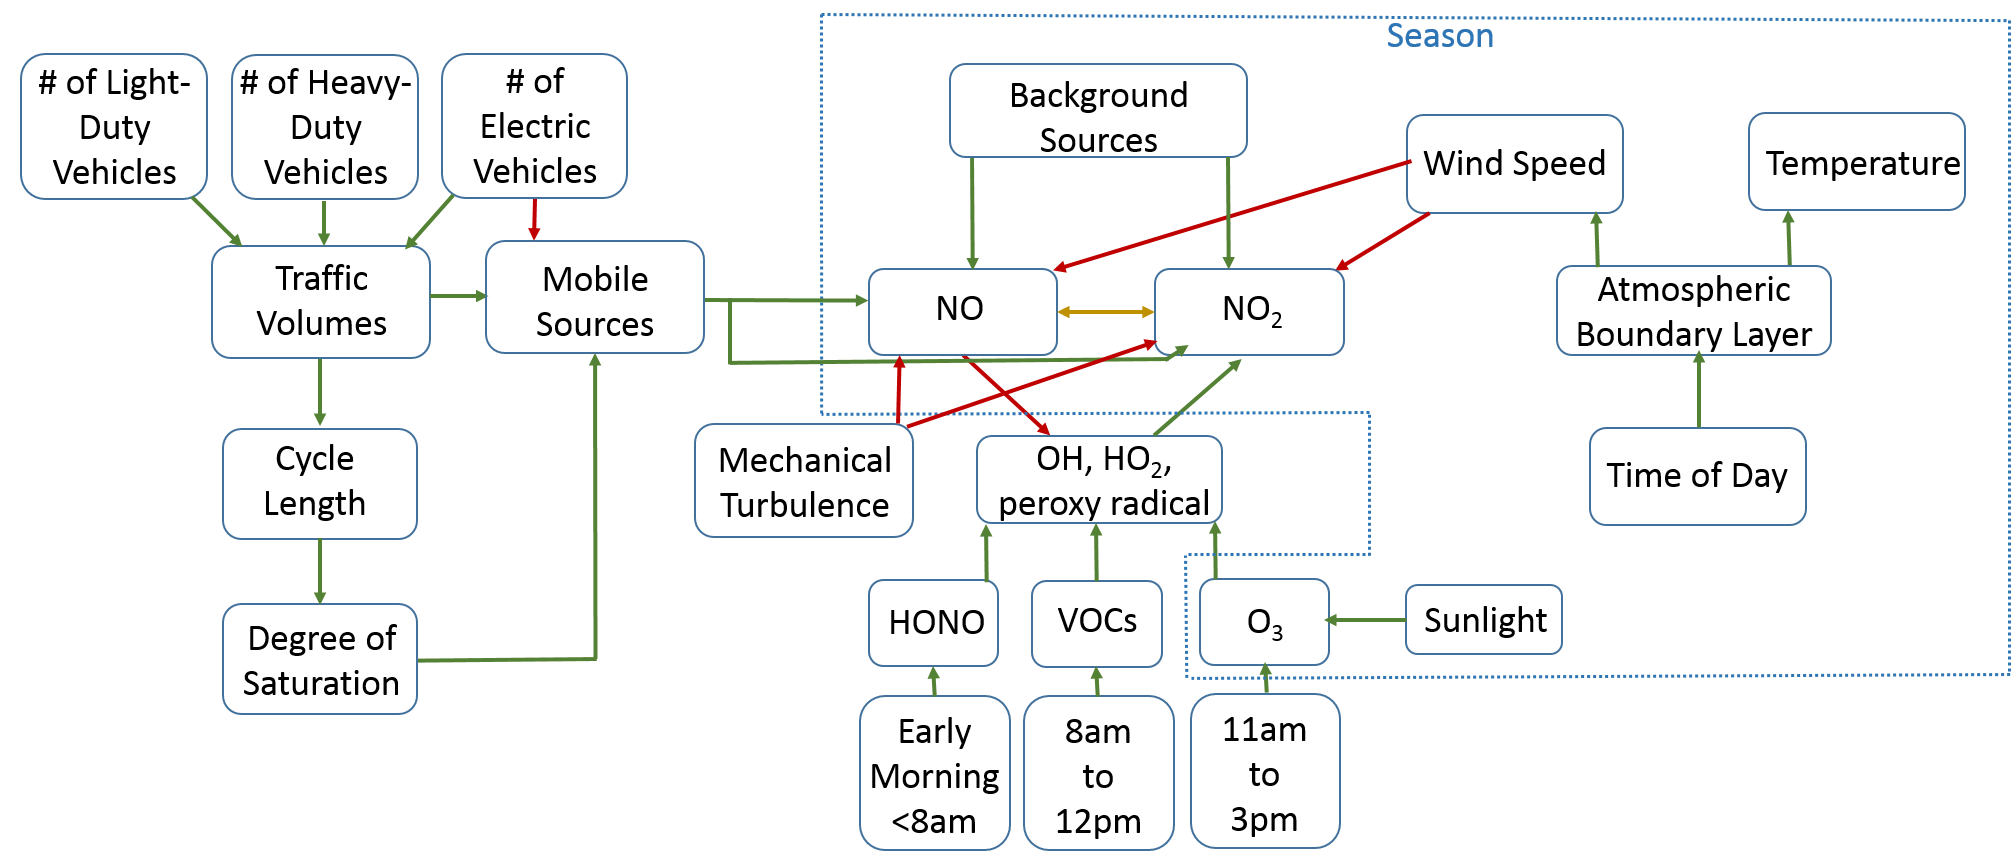
\includegraphics[width=\linewidth]{portland}
\end{figure}

This diagram correlates the measurement variables of an air pollution monitoring system with other, partially-observable variables like traffic composition, mechanical turbulence, and the presence of sunlight. It presents an intuitive and apparently useful description of a system at large. We would like to clarify the meaning of this diagram, and of others like it, by giving its interconnections a precise mathematical meaning. Clarifying the meaning of the diagram will not only make it more useful; it will allow us to connect this local, correlation-based picture of a system with other local pictures, as well as with more sophisticated scientific models of the world.

% Next paper: In this paper, we will present an easy, plug-and-play approach to combining models with data. We reference a previous paper, indicator frameworks, as one instantiation of a much larger framework: that of mapping mathematical models to data models. For example, algebraic quantum field theories similarly take a causal structure and map it via functor to a category of $C^*$-algebras, which encode the possible observations for that causal structure. In natural language, distributional compositional models of meaning map a pregroup to vector-space models of language, which (usually) encode observations of words within a corpus.

% While we discuss several directions for generalizing this work in \cref{sec:discussion}, we emphasize a correlation-based data model in order to emphasize the simplicity and elegance of the approach, especially in practical applications.

In this paper, we develop \emph{abstract indicator frameworks}, a mathematical tool for interpreting and combining systems of random variables and their correlations. Abstract indicator frameworks are modeled off operational (key performance) indicator frameworks, especially as they are used in city planning and project governance. Such operational indicator frameworks have three main uses: (1) to communicate quantitative information and strategic priorities to a wide audience, (2) to enable policy reactions to data, especially in the optimization of processes, and (3) to restrict attention to a set of `relevant' indicators---thus discarding the information from many other, `non-relevant' indicators. % In this paper, we will focus on (3), i.e. on relevance, since it is conceptually prior to (1) and (2). Talking about relevant indicators is just another way of talking about how to construct an indicator framework.

In city planning, there are several strategy-setting frameworks for constructing operational indicator frameworks, from balanced scorecards \cite{epstein1997balanced} to SMART \cite{doran1981there} to more specialized urban planning frameworks; in such frameworks, the indicators are often designed by mayors, chief strategy officers, and sizable expert committees in tandem with new projects, new policies, and new processes. Even assuming that the participants adhere to a framework, the process of choosing indicators is often ad hoc, the choice of indicators does not account for pre-existing statistical relationships between the indicators, and integrated data for all such indicators can be hard to capture. Once built, the indicator frameworks for cities also tend to be large and unwieldy: there are 175 indicators in the CITYkeys standard \cite{citykeys??} and 212 in the Boston Indicators Project \cite{bostonindicators??}. (And there are already more than 43 indicator frameworks built for ``smart and sustainable cities'' alone!) The point: indicator frameworks can be useful locally, but they are hard to build at scale, hard to sustain at scale, and hard to use at scale.

% Even CityScore in Boston, one of the pioneering efforts beh, has been criticized for its lack of transparency and lack of usefulness.

We propose an alternative: ``start with the data you have, not the data you want''. Instead of constructing operational indicator frameworks expensively and internally, meaning indicator-by-indicator, we can specify them abstractly and externally, by means of their causal and statistical relationships to other, already-extant sets of indicators. Our approach is especially suited to situations where heterogeneous measurement data is distributed across many projects, many subject domains, and many localities, as in a city.
 
Correlation table!
\[
\begin{tabular}{c|ccccc}
		& $A$ & $B$ & $C$ & $D$ & $E$ \\ \hline
$A$		& 1 & 0.1 & -0.8 & \hl{$x_1$} & \hl{$x_2$} \\
$B$		& & 1 & 0.2 & \hl{$x_3$} & \hl{$x_4$} \\
$C$		& & & 1 & 0.9 & -0.3 \\
$D$		& & & & 1 & -0.7 \\
$E$		& & & & & 1
\end{tabular}
\]
 
However, such an approach faces several practical data-engineering challenges:
\begin{problem}[Data integration]
It is not always possible to directly compare local sets of indicators---e.g. to construct a correlation matrix---especially when the indicator sets are disjoint. The combined data over all the indicators may not exist; or if the data does exist, it may not be sufficient to support the kinds of arguments the user wants to make; or it may be prohibitively difficult to integrate the data for a multitude of different reasons \cite{halevy_integration_book?}.
\end{problem}
% (Though, in principle, we can generalize to other types of data models, such as database schemas or formal languages.)
\begin{problem}[Model integration]
The abstract approach fundamentally limits our ability to choose the right indicators. We are given observational data that is presumed sufficient to manage some local systems of interest, like a bus line or a classroom, but this data cannot usually capture all the possible causal interactions between the variables of a larger system, e.g. transportation \emph{and} education in the City of Boston. Managing---not solving---this problem requires that we supplement the missing data with background knowledge about the larger system under study. But such knowledge, like the data, tends to arrive modularly, over the local systems in question. So we need not only the background knowledge, but also a way to stitch different models together. % We model this problem of model integration in a category of causal models, $\Caus$. 
% (Though, in principle, we can generalize to other types of scientific models, such as Bayesian networks or dynamical systems.)
\end{problem}
\begin{problem}[Compositional semantics]
An operational account of indicator frameworks needs to tell us not just what they are, but how they are \emph{used}. To us, this is a question of semantics: the way we use an indicator---the kind of arguments we make with it---depends on how we interpret its meaning, and this meaning is governed by installing a mathematical model over the data. % We model this semantics as a functor from $\Caus$ to $\Rand$.
\end{problem}

% For example, cities are often interested in understanding the second-order impacts of specific projects, e.g. the impacts on health, crime, and jobs of a smart shuttle system. Assuming the existence of a local indicator framework for the shuttle system, and the existence of a top-level indicator framework representing broad priorities such as health, crime, jobs, and so on, then we can construct a mediating indicator set whose indicators satisfy certain statistical and causal relationships generated by the given indicator frameworks; these mediating indicators represent the second-order impacts of the local project to the city's other priorities.

These three problems motivate the definition of abstract indicator frameworks. An operational indicator framework is a list of indicators along with an account of how these indicators are used. An abstract indicator framework is, roughly, a formula for turning ``scientific models'' into spaces of random variables. (Such frameworks may be compared with the usual algorithms for using data to construct a scientific model.) But an abstract indicator framework can also be understood as an object on its own, rather than as a formula; in particular, it is possible to define maps and gluings between different abstract indicator frameworks. We will apply \emph{category theory}, originally developed to relate and analyze topological spaces, as an efficient language for relating and analyzing the causal and statistical aspects of abstract indicator frameworks. To illustrate the mathematics, we will develop a running example of how a mayor can implement the approach.

% This motivates the definition of abstract indicator frameworks, which we define as the objects of a certain ``category of diagrams of random variables'', $\Ind$. 

% we should have a story for how to abstract away processes we don't model (like social ones) ``into the data''

\subsubsection{Notation}
Let $\mathcal{X}$ stand for an indicator set. Abstract indicator frameworks have a notion of \emph{process} that transforms one indicator set into another, a notion of \emph{state} that represents the process of picking a specific indicator in $\mathcal{X}$, and a notion of \emph{effect} that represents the process of ``measuring'' or computing the correlation with respect to a specific indicator in $\mathcal{X}$. Processes, states, and effects are represented, respectively:
\[
\begin{tikzpicture}
	\begin{pgfonlayer}{nodelayer}
		\node [style=none] (0) at (-5, -1) {};
		\node [style=none] (1) at (-5, 1) {};
		\node [style=box] (6) at (-5, 0) {$f$};
		\node [style=point] (2) at (0, -0.5) {$X$};
		\node [style=none] (4) at (0, 1) {};
		\node [style=none] (3) at (5, -1) {};
		\node [style=copoint] (5) at (5, 0.5) {$Y$};
	\end{pgfonlayer}
	\begin{pgfonlayer}{edgelayer}
		\draw [style=none] (1.center) to (0.center);
		\draw [style=none] (2) to (4.center);
		\draw [style=none] (5) to (3.center);
	\end{pgfonlayer}
\end{tikzpicture}
\]
These are needed to capture the operations of composing processes in sequence, called \emph{composition}, and combining them in parallel, called \emph{tensoring}. The composition $g \circ f$ (first $f$, then $g$) and tensor $f \otimes g$ are represented as:
\[
\begin{tikzpicture}
	\begin{pgfonlayer}{nodelayer}
		\node [style=box] (0) at (-3, -1) {$f$};
		\node [style=none] (1) at (-3, 2) {};
		\node [style=box] (2) at (-3, 1) {$g$};
		\node [style=none] (3) at (3, 1) {};
		\node [style=box] (4) at (3, 0) {$f$};
		\node [style=none] (5) at (3, -1) {};
		\node [style=none] (6) at (-3, -2) {};
		\node [style=none] (7) at (4.5, -1) {};
		\node [style=box] (8) at (4.5, 0) {$g$};
		\node [style=none] (9) at (4.5, 1) {};
	\end{pgfonlayer}
	\begin{pgfonlayer}{edgelayer}
		\draw [style=none] (1.center) to (0);
		\draw [style=none] (3.center) to (5.center);
		\draw (0) to (6.center);
		\draw [style=none] (9.center) to (7.center);
	\end{pgfonlayer}
\end{tikzpicture}
\]

We call any formalism with a notion of composition and tensoring a \emph{process theory}. The semantics of process theories and their diagrams are governed by the theory of monoidal categories, which is surveyed in \cite{selinger09}. The goal of the paper is to specify an appropriate symmetric monoidal category, $\Rand$, representing the appropriate operations on random variables, after which we can define a causal model as a strong monoidal functor from a causal theory into $\Rand$. These causal models---essentially, diagrams in $\Rand$---will be the promised abstract indicator frameworks. In \ref{??3.1}, we will consider a preliminary version of $\Rand$ along with some of the possible alternatives. In \ref{?? 3.2}, we will give the statistical justification for our choice of $\Rand$, review the notion of a causal model from \cite{fong13}, and then give the full definition of abstract indicator frameworks.

% footnote{There's a slightly philosophical discussion here as to whether the best approach to complex causal modeling is to define a causal theory $\mathcal{C}$ first, as in \cite{fong13}, and then to define causal models as monoidal functors \emph{out of} $\mathcal{C}$, or to define an appropriate ``working category'' $\mathcal{D}$ first, then see what sorts of causal and scientific models one can define \emph{into} $\mathcal{D}$. Our intuition is that, while it will take some time to nail down the appropriate working category---e.g. between $\Bayes$, $\Stoch$, or the proposed $\Ind$---the number of useful and possible causal and scientific models will actually vary far more, in practice, than the number of viable working categories.} 

% Intuitively, a strong monoidal functor into $\Rand$ captures the idea of ``scientific model with respect to data''.

\section{Background}
As mentioned above, there are a variety of approaches to choosing indicator frameworks as part of the process of strategic priorities. Of the many specialized approaches to choosing indicator frameworks in various fields, Niemejer and de Groot \cite{niemeijer08} have suggested a similar methodology for choosing environmental indicator sets based on explicit causal networks of environmental forces and societal response; while their methodology is still largely qualitative rather than formal or statistical, their paper handily illustrates how (diagrams of) causal models can facilitate the selection of relevant indicator sets. % In statistics, Horvath \cite{horvath11} also takes a compositional approach to correlation by focusing on weighted correlation networks, which represent random variables by nodes in a graph and edges between variables by a soft threshold on their correlation. These correlation networks have proved useful for analyzing high-dimensional data sets, especially gene expression data.

% Compare indicator frameworks to ``interpretable'' models in data science?

\redout{Relate to ``conceptual spaces'' idea in Bob's work as well as in the original Gardenfohrs, since we are depending very much on Hilbert spaces to store the geometry of our data.}

\redout{A related idea... can we understand correlation as signifying or approximating a kind of ``cooperation'' between variables? Think about what it represents in higher-order phenomena: what's happening between two things at many levels. The level of cooperation can be used to summarize a single system.}

\redout{For completeness, we provide the following definition from \cite{pearl09}.

\begin{definition}[Causal Bayesian network] Let $P(v)$ be a probability distribution on a set $V$ of random variables, and let $P(v|do(x))$ denote the distribution resulting from the intervention $do(X = x)$ that sets a subset $X$ of variables to constants $x$. Denote by $P_\ast$ the set of all interventional distributions $P(v|do(x))$ for all $X \subset V$, including $P(v)$, which represents $X = \O$. A DAG $G$ is said to be a causal Bayesian network compatible with $P_\ast$ if and only if the following three conditions hold for every $P(v|do(x)) \in P_\ast$:
\begin{enumerate}
\item $P(v|do(x))$ is Markov relative to $G$.
\item $P(v_i|do(x)) = 1$ for all $V_i \in X$ whenever $v_i$ is consistent with $latex X = x$.
\item $P(v_i|do(x), pa_i) = P(v_i | pa_i)$ for all $V_i \notin X$ whenever $pa_i$ is consistent with $X =x$.
\end{enumerate}
Causal Bayesian networks are to be distinguished from the standard ``associational'' Bayesian networks, since they are defined explicitly in terms of post-interventions distributions.
\end{definition}
}

% \redout{[TO ADD: Pearl's discussion of causality and causal models using diagrams, methods of doing observational studies by eliminating interventions = surgeries on equations via diagrams. Simpson's paradox (see Fong's example).]}

% \redout{[Other things: structural equation modeling and construct validity, ref. Petter 2007 or Churchill 1979, where constructs are structural and measurement models used in the study of systems, e.g. as in structural equation modeling. Also, stress-condition-response models, which are mentioned in Niemejer as well.]}

Even within the constraints of a process theory, there are still a number of approaches to formalizing probability. In this section, we will go over three examples: the Hilbert space interpretation of random variables, the original category of probabilistic mappings suggested by Lawvere \cite{lawvere62}, and the diagrammatic approach of Coecke and Spekkens \cite{coecke_spekkens} to Lawvere's work. \redout{Also discuss the approach, in quantum physics, of mapping various models into categories of $C^\ast$-algebras. In particular: an algebraic quantum field theory is where you take a causal theory structure and map it to some $C^\ast$-algebra.} We also briefly discuss graphical models such as those surveyed in \cite{lauritzen96}, which are the most obvious applications of \cite{lawvere62} and \cite{coecke_spekkens}, e.g. see \cite{fong13}.

The Hilbert space interpretation, which we call $\Rand$, uses the fact that real-valued random variables over some fixed probability space $(\Omega, \mathcal{F}, \mathbb{P}$) form a Hilbert space $H$ where the inner product $\langle X, Y \rangle$ is just the covariance $\mathbb{E}(XY)$. Assuming that we restrict ourselves to standard variables with zero mean and unit variance, the covariance equals the correlation, and we can represent both by the inner product in $\Rand$.  This inner product can be represented by a process diagram, namely as the composition of a state and an effect in $\Rand$:
\[
\Cor(X,Y) = \text{Cov}(X,Y) = \langle X, Y \rangle =
\begin{tikzpicture}
	\begin{pgfonlayer}{nodelayer}
		\node [style=point] (0) at (0, -1) {$X$};
		\node [style=copoint] (1) at (0, 1) {$Y$};
	\end{pgfonlayer}`
	\begin{pgfonlayer}{edgelayer}
		\draw [style=none] (1) to (0);
	\end{pgfonlayer}
\end{tikzpicture}
\]
As we will see in the next section, $\Rand$ is actually already very close to what we want; the problem is that the obvious categorical interpretation of $\Rand$ does not give a natural way of analyzing the data of ``intermediate'' correlations.

$\Rand$ is closely related to older work on the categorical foundations of probability initiated by Lawvere in \cite{lawvere62} and developed in Giry \cite{giry82}:
\begin{definition}
The category $\Stoch$ of stochastic processes is defined by the following data:
\begin{enumerate}
\item objects are measurable spaces $(A, \Sigma_A)$ of sets $A$ with a $\sigma$-algebra $\Sigma_A$
\item morphisms $P : (A, \Sigma_A) \to (B, \Sigma_B)$ are stochastic kernels, i.e. functions $P : A \times \Sigma_B \to [0,1]$ that assign to $(a, \sigma_B)$ the probability of $\sigma_B$ given $a$, denoted $P( \sigma_B | a)$ % such that $\sum_{y \in \Sigma_B} X(a, y) = 1$
\item composition $Q \circ P : A \times \Sigma_C \to [0,1]$ of $P : (A,\Sigma_A) \to (B,\Sigma_B)$ and $Q: (B,\Sigma_B) \to (C, \Sigma_C)$ is defined by \[(Q \circ P)(\sigma_C | a) = \int_{b \in B} Q(\sigma_C | b) dP_a,\] i.e. marginalization over $B$
\end{enumerate}
\end{definition}

As suggested by the notation, morphisms in $\Stoch$ represent probability measures on an event/outcome space $(A, \Sigma_A)$. If we restrict to the subcategory $\FinStoch$ whose objects are \emph{finite} measurable spaces---since the outcomes are finite, one can imagine these spaces as sets of natural numbers $\{1, ..., n\}$---then we can think of stochastic kernels are stochastic matrices, i.e. matrices whose column entries sum to 1. Taking $1 = (\{\ast\}, \Sigma_\ast)$ as the monoidal unit, we can see that a probability distribution in $\FinStoch$ is just a vector $P : 1 \to (A, \Sigma_A)$ whose entries are the probabilities of all the possible atomic outcomes in $A$. The usual tensor product described in $\Stoch$ is the functor $\otimes: \Stoch \times \Stoch \to \Stoch$ that assigns to two probability distributions $P : 1 \to (A, \Sigma_A)$, $Q : 1 \to (B, \Sigma_B)$ their product measure, i.e. the map $PQ : 1 \to (A \times B, \Sigma_A \otimes \Sigma_B)$ s.t. $PQ(\ast, (a,b)) = P(\ast,a) Q(\ast, b)$.

Using the language of symmetric monoidal categories, Coecke and Spekkens \cite{coecke_spekkens} give a graphical calculus for $\FinStoch$ and use it to elaborate Bayesian reasoning (in particular, a diagrammatic representation of Bayes' rule). As above, objects of $\FinStoch$ are natural numbers, morphisms from $m$ to $n$ are $n \times m$ stochastic matrices, composition is matrix product, and the monoidal product is the matrix tensor product. States are probability distributions over the set ${1, ..., n}$:
\[
\begin{tikzpicture}
	\begin{pgfonlayer}{nodelayer}
		\node [style=point] (0) at (0, 0) {$P$};
		\node [style=none] (1) at (0, 1) {};
	\end{pgfonlayer}
	\begin{pgfonlayer}{edgelayer}
		\draw [style=none] (1) to (0);
	\end{pgfonlayer}
\end{tikzpicture}
: 1 \to A = (p_1, ..., p_n) \text{ such that } \sum_{j=1}^n p_j = 1
\]

A \emph{joint state} is a state over the composite object ${1, ..., mn}$, of the form
\[
\begin{tikzpicture}
	\begin{pgfonlayer}{nodelayer}
		\node [style=wide point] (0) at (0, 0) {$P$};
		\node [style=none] (1) at (0.75, 1) {};
		\node [style=none] (2) at (0.75, 0) {};
		\node [style=none] (3) at (-0.75, 1) {};
		\node [style=none] (4) at (-0.75, 0) {};
	\end{pgfonlayer}
	\begin{pgfonlayer}{edgelayer}
		\draw [style=none] (1) to (2);
		\draw [style=none] (3) to (4);
	\end{pgfonlayer}
\end{tikzpicture}
\]
A joint state is ``uncorrelated''---one should be careful, since this is correlation between probability distributions, not between random variables per se---when it can be decomposed into a tensor product, and perfectly correlated when it can be represented as a delta function. Uncorrelated and perfectly correlated joint states are depicted, respectively:
\[
\begin{tikzpicture}
	\begin{pgfonlayer}{nodelayer}
		\node [style=point] (0) at (0, 0) {$P$};
		\node [style=none] (1) at (0, 1) {};
	\end{pgfonlayer}
	\begin{pgfonlayer}{edgelayer}
		\draw [style=none] (1) to (0);
	\end{pgfonlayer}
\end{tikzpicture}
\;
\begin{tikzpicture}
	\begin{pgfonlayer}{nodelayer}
		\node [style=point] (0) at (0, 0) {$Q$};
		\node [style=none] (1) at (0, 1) {};
	\end{pgfonlayer}
	\begin{pgfonlayer}{edgelayer}
		\draw [style=none] (1) to (0);
	\end{pgfonlayer}
\end{tikzpicture}
: 1 \to A \otimes B = (p_1q_1, ..., p_nq_m) % \text{ such that } \sum_{i=1}^{n} \sum_{j=1}^m p_iq_j = 1
\]
\[
\begin{tikzpicture}
	\begin{pgfonlayer}{nodelayer}
		\node [style=small black dot] (0) at (0, -0.5) {};
		\node [style=none] (1) at (1, 0.5) {};
		\node [style=none] (3) at (-1, 0.5) {};
	\end{pgfonlayer}
	\begin{pgfonlayer}{edgelayer}
		\draw [style=none, bend left=45] (1) to (0);
		\draw [style=none, bend left=45] (0) to (3);
	\end{pgfonlayer}
\end{tikzpicture}
: I \to A \otimes A = (\delta_{i,i'} \in \{1, ..., n\}.
\]
A perfectly anti-correlated joint state in $\FinStoch$ is just a cup with a NOT-gate attached to one end. 
%\begin{figure}[h!]
%\centering
%\label{bob_anticorrelated_state}
%
\includegraphics[width=\linewidth]{bob_correlated_state}
%\end{figure}
More generally, any correlation can be obtained by attaching a suitable box to one of the ends of the cup.

There are two major problems with this graphical formalism, and with $\Stoch$ and $\FinStoch$ in general. First and foremost, there is not a very convenient way of talking about \emph{random variables}. Technically, a real-valued random variable is given by the diagram below, of a measurable function $X : (\Omega, \Sigma_\Omega) \to (\mathbb{R}, \Sigma_\mathbb{R})$ which takes possible outcomes in $\Omega$ to their numerical representations in $\mathbb{R}$ (technically, $X$ is not a function but a stochastic matrix whose columns represent point probabilities), a probability measure $P : 1 \to (\Omega, \Sigma_\Omega)$ on the outcomes in $\Omega$, and finally the pushforward $X(P)$ of $P$ along $X$, which represents the probability distribution of the random variable $X$.
\[
\begin{tikzcd}
1 \arrow[r, "P"] \arrow[rd, "X(P)"'] & (\Omega, \Sigma_\Omega) \arrow[d, "X"] \\
 & (\mathbb{R}, \Sigma_\mathbb{R})
\end{tikzcd}
\]
Besides being difficult to work with, the point of view of this paper is that probability measures are not random variables nor are they sufficient replacements; a probability measure is something probability theorists invented in order to talk about random variables. While useful in the context of Bayesian networks, which can be articulated primarily in terms of stochastic processes, probability measures are less visible in cases driven by data and by correlational arguments.

The second problem is that there is not a good interpretation of \emph{effect}, i.e. of ``measuring'' or computing something with respect to a specific state. An effect in $\FinStoch$
\[
\begin{tikzpicture}
	\begin{pgfonlayer}{nodelayer}
		\node [style=none] (0) at (0, 0) {};
		\node [style=copoint] (1) at (0, 1) {$X$};
	\end{pgfonlayer}
	\begin{pgfonlayer}{edgelayer}
		\draw [style=none] (1) to (0);
	\end{pgfonlayer}
\end{tikzpicture}
\]
is defined to be a morphism $X^\dagger : (A,\Sigma_A) \to 1$, i.e. a function $X^\dagger : A \times \Sigma_\ast \to [0,1]$. The problem is that $1$ is terminal in $\Stoch$: there is only one possible morphism from any object to 1 due to the constraint on morphisms of being a probability measure. In particular, for any $(A, \Sigma_A)$ and for all $a \in A$, the unique map $X^\dagger : (A, \Sigma_A) \to 1$ is given by $X^\dagger(\ast | a) = 1$ and $X^\dagger( \varnothing | a) = 0$. In other words, any `measurement' of a state (i.e. a probability distribution) in $\FinStoch$ and $\Stoch$ simply kills the state. % Essentially, $X^\dagger$ represents a random variable, since $X^\dagger(\ast | a)$ is just the probability of $A$ $\ast$ given $a$. But $X^\dagger \circ X (\ast | a)$ functor returns a probability for each element of $A$, so it amounts to a random variable.

In Bayesian statistics and machine learning, graphical models have been developed to model the conditional (in)dependence of systems of random variables; the joint distribution over all the random variables in a graphical model is the product of their conditional distributions. Among the most familiar examples of graphical models are (directed) Bayesian networks and (undirected) Markov networks. The upshot is that complex questions about joint distributions of many interrelated variables can be answered in terms of the topology of the graph. Graphical models, Bayesian networks, stochastic matrices ground several existing mathematical approaches to integrating causality with probability, including that of $\Stoch$ and $\FinStoch$ \cite{coecke}. The study of causality in probability has deeper roots in structural equation modeling and Pearl's work on the do-calculus \cite{pearl09}. % [Need more explanation and figures.]

% Typically, in such a diagram one begins with some states, which are the prior probabilities, and then transforms these through a given protocol---representing sampling from a distribution---to end up with new states, which are the posterior probabilities.

% One criticism of $\Stoch$, and by extension $\Bayes$, is that by focusing measure spaces and stochastic maps, they miss the fact that probability theory is not really about probability spaces; it is about families of random variables.

% $\Bayes$, $\Stoch$, and graphical models such as Bayesian networks give a semantics for probabilistic reasoning, but even when they do not explicitly represent causal models of the world, their underlying idea---conditional dependence---is at its core a formal method for causal inference. In scientific inquiry, where the explanatory power of theories is valued at a premium, this counts as a major advantage over correlation-based approaches, which are less abstract and live closer to the data. \redout{But therein lies the problem: causal models are useful for interpreting the results of a scientific experiment, but they are not useful, generally speaking, when the data do not provide evidence for causation, such as in observational studies of complex systems. We want to carefully distinguish the causal aspects of our models from their non-causal aspects, and the first step is to develop a coherent framework for \emph{non-causal} reasoning. THIS ISN'T TRUE. Causal models are incredibly useful for interpreting observational studies, since you need it to disambiguate confounding variables. However, this is a local activity. How can we determine the }

% more positive way of describing non-causal: what it means to have a status quo... everything is different, yet everything is more or less the same.
% The key distinction between a causal and a non-causal theory is that, in a causal theory, the state of one variable (e.g. a `parent variable' in a graphical model) can be used draw inferences about or `condition' another variable (e.g. a `child variable' in a graphical model), and in a non-causal theory, one cannot draw such inferences. This is a more positive way of characterizing non-causal theories, which we describe in the next section. 

% \redout{A third approach fixes a specific Hilbert space of random variables and interprets it as a Lawvere metric space. But is there a monoidal product in this space? Even if not, and there is no graphical interpretation, would there still be a reason to do this?}

\section{Method}
In this section, we describe how to construct, use, and compare abstract indicator frameworks, at each step giving both the operational and the mathematical specification.

\subsection{Constructing indicator frameworks}
Here is a step-by-step guide to constructing an abstract indicator framework.

\begin{enumerate}
\item Take as input a list of $\mathbb{R}$-valued random variables, representing indicators, and a correlation matrix between them.
\item Construct a finite-dimensional vector space $N$ with the original random variables as basis elements. The inner product between basis elements $i,j$ should match the value of the $i,j$-th entry in the correlation matrix. % representing the ``noun space'' of the variables
\item Separately, define a scientific model over those random variables. % representing a ``sentence'' over your nouns. 
For example, $X \to Y \leftarrow Z$ is a causal model of (causal) variables $X, Y, Z$.
	\begin{enumerate}
	\item Divide the basic components $s_i$ of your scientific model into types or ``grammatical roles''. For example, a causal model has only two types: causal variables and arrows. % , and assign to each type a string of symbols $p_1 ... p_m$. , where variables are assigned the string $n$, and arrows are assigned the string $nsn$.
	\item Define the grammatical rules for how types can be composed. For example, an arrow in a causal model is only grammatical when it appears between two causal variables.
	\end{enumerate}
\item Assign each type in your scientific model to a vector space. In a causal model, variable types go to the vector space $N$ and causal arrows go to $N \otimes S \otimes N$, where $S$ is the one-dimensional $\mathbb{R}$-vector space with $\vec 0$ as origin and $\vec 1$ as basis element. (In general, $S$ can be any vector space.) For example, the causal model $A \to B$ has type $N \otimes (N \otimes S \otimes N) \otimes N$.
\end{enumerate}

We will see an example of this in Section~\ref{???}.

The types in the scientific model correspond to types of sentences. So, really, any shape of causal diagram should be an object in Caus!

The sentence space could be $is_surprising \times is_positive$.

\subsection{Using indicator frameworks}
Having constructed an abstract indicator framework, $F$, we can now use it.

\begin{enumerate}
\item Construct an embedding $\sigma$ from the components $s_i$ of your scientific model into the vector space corresponding to the type of that component. In a causal model, $\sigma$ is fixed by the definition of $N$, while the causal arrow $\to$ maps to the vector $\vec \Psi$ in $N \otimes S \otimes N$ given by 
\[ \vec \Psi = \sum_{i,j,k} c_{ijk} (n_i \otimes s_j \otimes n_k) \in N \otimes S \otimes N \]
where $c_{ijk} = 1$ when $n_i$ causes $n_k$, and 0 otherwise. So we have directly defined the embedding by encoding each component $s_i$ within the basis of its target vector space. More generally, one can apply machine learning methods to a large corpus of data in order to construct such an embedding $\sigma$.
\item Using the embedding above, embed each component $s_i$ of your scientific model in order to obtain a ``linearized'' version of that model, $v_1 \otimes ... \otimes v_m \in V_1 \otimes ... \otimes V_m$.

% though we assume that in ``local'' models, the direct encoding is known.

% The ``meaning'' of a variable is just its relative position compared to all the other variables.

\item Choose a \emph{type reduction} $F(f) : V_1 \otimes ... \otimes V_m \to U_1 \otimes ... \otimes U_k$. 
% $ f : p_1 ... p_n \to q_1 ... q_m$ 
For example, given a causal model $A \to B$, we can define a reduction $F(f) : N \otimes (N \otimes S \otimes N) \otimes N \to S$ by $F(f) = \epsilon_N \otimes 1_S \otimes \epsilon_N$ where $\epsilon_N : N \times N \to \mathbb{R}$ is the inner product map $\langle - | - \rangle$ (a.k.a. the co-unit).

\item Apply $F(f)$ to your vector $v_1 \otimes ... \otimes v_n$. The result, in the reduced vector space, is the ``meaning'' of the scientific model in the form of a single random variable.
\end{enumerate}

\begin{table}[tbh]
\label{table:ML_glossary}
\begin{center}
\begin{tabular}{l | p{10cm}}
term & semantics \\ \hline
scientific model & an object in an autonomous category \\
causal model & an object $C \in \Caus$ \\
indicator framework & functor $F : \Caus \to \Rand$ \\
%empirical risk minimization & a paradigm \\
%maximum margin & a paradigm \\
%maximum entropy \\
%maximum likelihood \\
%statistical convergence \\
%uniform convergence
\end{tabular}
\end{center}
\caption{A glossary of basic mechanisms for describing the behavior of a learning algorithm $A$ with hypothesis $h$ on a given (labeled) data set $S$.}
\end{table}

% How do we get ``data'' into the category of convex relations? Take the example of the birdsong experiment. A neural network learns the manifold of birdsongs from many examples, and interpolates between different clusters (first, I think, it projects to a lower-dimensional space?). The birds are the ``discriminators'' which mark / distinguish different clusters in the space of all birdsongs. The clusterings are objects in ConvexRel? Perhaps we can integrate data by iteratively constructing different objects in ConvexRel via the training process. So the training procedure passes through the category in that way.

Roughly:
\[
\begin{tikzcd}[column sep=small]
& \text{System} \arrow{dr}{h} \arrow{dl}{g} & \\
\text{Scientific Model} \arrow{rr}{F} & & \text{Data Model} 
\end{tikzcd}
\]

An operational account of indicator frameworks should describe not only the data model but how we \emph{use} that data model. Our contention: we \emph{use} that data model in ways that are approximated by the scientific models inside our heads. 

Any meaningful scientific model is composed of parts, each of which has a meaning.

\redout{In general, it is not possible to identify a causal model uniquely. But neither is this the problem that we want to solve. Instead: how do we ``value'' the data of one system with respect to the data of another system? Alternately: how do we compare systems of variables with other systems of variables?}

Mathematically: \redout{Put into 2-column format.}

\begin{enumerate}
\item Using indicator data, specify an object $A$ in the data category $\Rand$. 
\item \redout{This is a rather subtle point. E.g. see \url{http://math.ucr.edu/home/baez/quantum/node3.html}.}
\item Pick an object in your grammar category, $\Caus$.
\item Define the objects of the grammar category of your scientific model, e.g. the category of causal models $\Caus$.
\item Define a strict monoidal functor $F : \Caus \to \Rand$.
\item Define a morphism $\sigma$ in $\Rand$ from the unit object to $A$.
\item Consider the morphism $\sigma$ as a generalized element.
\item Choose a morphism $f$ in $\Caus$.
\item Consider $F(f)$.
\item Consider $F(f) \circ \sigma$.
\end{enumerate}

Recall that real-valued, square-integrable random variables over a given probability space form a Hilbert space $L^2(\Omega, \Sigma, \mathbb{P})$ whose inner product is just the covariance. % i.e. the `best estimate of $X$ using $Y$', i.e. the linear function of $Y$ which is closest to $X$, i.e. $a + bX$ for some $a$ and $b$.

\begin{definition}
The category of random variables, $\Rand$, is defined by the following data:
\begin{enumerate}
\item objects are finite-dimensional Hilbert spaces \[ \mathcal{X} = L^2(\Omega_\mathcal{X}, \Sigma_\mathcal{X}, \mathbb{P}_\mathcal{X})\] of square-integrable random variables (under the equivalence relation $X_1 \sim X_2$ if $\mathbb{P}_\mathcal{X}(X_1 = X_2) = 1$) with inner product $\langle X,Y\rangle = E(XY)$, defined over probability spaces $(\Omega_\mathcal{X}, \Sigma_\mathcal{X}, \mathbb{P}_\mathcal{X})$, with an associated basis $\mathcal{B}_\mathcal{X} = \{ X_1, X_2, ..., X_n \} \cup \One$, where $\One$ is the random variable with constant value 1. % and all simple linear regressions of $X_i$ with respect to $X_j$
\item morphisms $F: \mathcal{X} \to \mathcal{Y}$ are bounded linear operators
% the cross-correlation matrices between (a vector of) the basis elements of $\mathcal{X}$ and those of $\mathcal{Y}$ 
% lifts of a stochastic kernel from $(\Omega, \mathcal{F}, \mathbb{P})$
\item identity $1 : \mathcal{X} \to \mathcal{X}$ is the identity matrix.
\item the composition is the usual composition of bounded linear operators
%two cross-correlation matrices $F: \mathcal{X} \to \mathcal{Y}$ and $G: \mathcal{Y} \to \mathcal{Z}$ is defined on individual entries by \[\Cor(X,Z) = \frac{1}{n} \sum_{Y_k \in \mathcal{Y}}^n \Cor(X,Y_k) \Cor(Y_k,Z)\]
\item the tensor product of $\mathcal{X}$ and $\mathcal{Y}$ is the pushout over their joint support in $\Omega_\mathcal{X} \times \Omega_\mathcal{Y}$, with monoidal unit $\One$.

\end{enumerate}
\end{definition}

\begin{lemma}
$\Rand$ is a symmetric monoidal category with the above tensor.
\end{lemma}

We defer the proof of the lemma to the appendix.

The fact that $\Rand$ is a symmetric monoidal category is a strong constraint on the semantics of the data model. It also allows us to write down equations in $\Rand$ in the language of string diagrams \cite{selinger13}. \redout{[Placeholder here for statistical interpretation of $\Rand$.]} % \subsubsection*{Statistical interpretation}

\begin{definition}
An \emph{abstract indicator framework} $F$ is a strong monoidal functor 
\[ F : \Caus \to \Rand. \]
\end{definition}

\begin{example}
\[ F(A \to B \leftarrow C) = N \otimes N \otimes S \otimes N \otimes N \otimes N \otimes S \otimes N \otimes N \]
\end{example}

% The meaning of a variable is fixed by its ``context'', where context is just the set of random variables around it... but this is not enough context!

$\Rand$ and the notion of mediating framework supply the basic statistical foundation for a theory of indicator frameworks. We would now like to incorporate a causal foundation. There are several reasons for doing so. First: many statistical arguments, e.g. partial correlation, actually rely on an implicit choice of causal model---see discussions related to confounding and mediating variables by Pearl \cite{pearl09}, among others. For example, given three random variables $X, Y, Z$; the partial correlations $\rho_{XZ \cdot Y}$, $\rho_{XY \cdot Z}$, or $\rho_{YZ \cdot X}$ are all equally valid; which one we take as `true' depends on which of the following causal structures we believe is true:

\[
\begin{tikzpicture}
	\begin{pgfonlayer}{nodelayer}
		\node [style=none] (0) at (-1, 1) {$X$};
		\node [style=none] (1) at (0, -1) {$Y$};
		\node [style=none] (2) at (1, 1) {$Z$};
	\end{pgfonlayer}
	  \path[-stealth]
	  	(1) edge node {} (0)
		(1) edge node {} (2) ;
\end{tikzpicture}
\quad
\begin{tikzpicture}
	\begin{pgfonlayer}{nodelayer}
		\node [style=none] (0) at (-1, 1) {$Y$};
		\node [style=none] (1) at (0, -1) {$X$};
		\node [style=none] (2) at (1, 1) {$Z$};
	\end{pgfonlayer}
	  \path[-stealth]
	  	(1) edge node {} (0)
		(1) edge node {} (2) ;
\end{tikzpicture}
\quad
\begin{tikzpicture}
	\begin{pgfonlayer}{nodelayer}
		\node [style=none] (0) at (-1, 1) {$X$};
		\node [style=none] (1) at (0, -1) {$Z$};
		\node [style=none] (2) at (1, 1) {$Y$};
	\end{pgfonlayer}
	  \path[-stealth]
	  	(1) edge node {} (0)
		(1) edge node {} (2) ;
\end{tikzpicture}
\]
Second, many operational indicator frameworks are constructed based on experts' causal models of the indicators, e.g. as in \cite{niemeijer08} or as in the air pollution diagram shown at the very beginning of this paper. Any story of indicator frameworks would be incomplete without mentioning causation. And third, the pattern developed here for causation will be useful later, when we want to incorporate not only causal models but arbitrary scientific models (such as those in Bayesian networks) into our indicator frameworks.

% How do we actually use this thing? Can we articulate a particular causal pathway of correlations, so that the optimal indicator framework between $X$ and $Z$ can be evaluated based on the causal structure.

% The need for a causal model is actually convenient, since we need to some way of structuring the optimization problem.

We recall the definition of causal theory from Fong \cite{fong13}, as a certain symmetric monoidal category induced from a directed acyclic graph (i.e. the causal structure), such as any of the three graphs above. Without going into the details, the idea is that given such a causal structure, we can specify a symmetric monoidal category whose objects are collections of the letters $\{X, Y, Z\}$, and whose morphisms are generated by the counit (representing `deletion') and comultiplication (representing `copying'), depicted respectively by
\[
\begin{tikzpicture}
	\begin{pgfonlayer}{nodelayer}
		\node [style=none] (0) at (-2, -1) {};
		\node [style=black dot] (1) at (-2, 1) {};
		\node [style=none] (2) at (2, -1) {};
		\node [style=none] (3) at (2, 0) {};
		\node [style=none] (4) at (1, 1) {};
		\node [style=none] (5) at (3, 1) {};
	\end{pgfonlayer}
	\begin{pgfonlayer}{edgelayer}
		\draw (1) to (0.center);
		\draw (3.center) to (2.center);
		\draw (3.center)[bend left=45] to (4.center);
		\draw (3.center)[bend right=45] to (5.center);
	\end{pgfonlayer}
\end{tikzpicture}
\]
and by a set of causal mechanisms generated from the causal structure, $[A] : \varnothing \to A$, $[B] : \varnothing \to B$, and $[C|AB] : AB \to C$, depicted as
\[
\begin{tikzpicture}
	\begin{pgfonlayer}{nodelayer}
		\node [style=point] (0) at (-4, -1) {$A$};
		\node [style=none] (1) at (-4, 1) {};
		\node [style=none] (2) at (0.5, -1.75) {};
		\node [style=none] (3) at (0.5, -0.5) {};
		\node [style=point] (4) at (-2, -1) {$B$};
		\node [style=none] (5) at (-2, 1) {};
		\node [style=none] (6) at (2.5, -0.5) {};
		\node [style=none] (7) at (1.5, 1) {};
		\node [style=large box] (8) at (1.5, -0.5) {$C | AB$};
		\node [style=none] (9) at (2.5, -1.75) {};
	\end{pgfonlayer}
	\begin{pgfonlayer}{edgelayer}
		\draw (1.center) to (0);
		\draw (3.center) to (2.center);
		\draw (5.center) to (4);
		\draw (7.center) to (8);
		\draw (6.center) to (9.center);
	\end{pgfonlayer}
\end{tikzpicture}
\]

Given a causal theory, i.e. a symmetric monoidal category, we can define a model of that causal theory $\mathcal{C}$ in $\Rand$ as a strong monoidal functor $F : \mathcal{C} \to \Rand$. To specify such a functor, it suffices to define its behavior on every atomic variable and every generating map in $\mathcal{C}$, i.e. the counit, comultiplication, and causal mechanisms of $\mathcal{C}$, since the values of the functor on the rest of $\mathcal{C}$ is specified up to isomorphism by the definition of a strong monoidal functor. For example, if $A$ is an atomic causal variable of the causal theory $\mathcal{C}$, then $F$ sends $A$ to a one-dimensional Hilbert space, e.g. one with basis set $\{X\}$. On tensor products of atomic causal variables, $F(A \otimes B)$ gives the tensor product $F(A) \otimes F(B)$, i.e. the space of random variables with basis set $\{F(A), F(B)\}$ and probabilities inherited from the product measure. On morphisms, $F([A]) : F(\ast) \to F(A)$ is just the single random variable in $F(A)$, and a causal mechanism $[C|AB]$ becomes a linear operator $F([C|AB]) : F(A \otimes B) \to F(C)$. % The comultiplication is just the diagonal map on 

Note that diagrams in the causal theory do not, typically, give rise to diagrams of the same shape in $\Rand$. For example, a confounding variable $Y$ with causal structure $X \leftarrow Y \to Z$ will typically generate the diagram corresponding to $\rho_{XZ\cdot Y}$. In general, each strong monoidal functor $\mathcal{C} \to \Rand$ converts a causal theory into a certain ``package'' of related indicator sets, where the operational indicator framework is represented by the terminal leaves of the causal theory. Picking the appropriate functor constitutes an optimization problem.

[Move to where?] So we lack data. But to take just one example, in a database setting there are ways to reason about ``missing data'', e.g. database nulls, especially when that data is the subject of a data migration or integration, as described in \cite{spivak10}. In particular, one can impose a set of algebraic equations that each null value must satisfy, where the equations are given by a diagram of database schema mappings. More generally, almost every diagram in a category articulates a set of constraints on the objects of that category.

\subsection{Comparing indicator frameworks}
Now, given two indicator frameworks $F: \Caus \to \Rand$ and $G : \Caus \to \Rand$, we can compare them in the following way:

Roughly: 

\[
\begin{tikzcd}[column sep=small]
\text{Scientific Model 1} \arrow{r}{i}  \arrow{d}{g} & \text{Grammatical Model} \arrow{dl}{k} \\
\text{Data Model} & \text{Scientific Model 2}  \arrow{l}{i} \arrow{u}{h}
\end{tikzcd}
\]

%\begin{enumerate}
%\item ???
%\item ???
%\item ???
%\end{enumerate}

\subsubsection*{An analogy}
Suppose that we are given a set of $n$ nouns, along with a word embedding of those nouns to a vector space spanning those words $\mathbb{R}^n$. Separately, someone has arranged (some of) those words into a sentence.

Suppose, now, that we have many such sets of nouns, and a sentence for each set of nouns. There may or may not be overlaps between the noun spaces, but we assume that the inner product (i.e. relative distance) between nouns is preserved across different embeddings. We assume that the sentences all belong to the same language (of, if you will, all the models are of the same ``type''), though really the only thing that matters is that the functor $F$ is defined on the verbs; i.e. the verbs have meaning.

The key question: how do I best arrange these sentences? Well... I cannot calculate correlations between words coming from different sentences directly; in other words, the embeddings are supposed to agree on their overlaps % I.e., the tensor $w_1 \otimes ... \otimes w_n \otimes v_1 \otimes ... \otimes v_n$ may equal zero if they have no joint support in the underlying data.

% Each causal link introduces a dummy variable? That would be a nice way to think of it... the causal links are themselves the ``sentence'' structure.

% Can we stitch back together the sentence, knowing the grammar?

% To do: describe the point of the normal tensor product for noncommutative rings, i.e. that it guarantees a unique factorization to any target, such that the triangle commutes.

% Optimization of processes depends on the variables being correlated or anti-correlated (i.e. not orthogonal). So we would expect that the correlation matrix of a local system be relatively far from the identity matrix.

% QUANTUM THOUGHTS
% Concretely, ``no global underlying reality'' means that there is not a well-defined joint distribution on ALL the variables. What's an example, in city planning, of a case where not all measurement events are simultaneously satisfiable, i.e. where the gluing of events is inconsistent? Consider a set of random variables, representing a local project. We can `glue' this set of variables with another set of random variables by saying that we can co-measure the two (we can generate integrated data sets).
% How related are the notions of correlation and ``superposition'' and entanglement in quantum mechanics?
% How do we define a measurement cover for a given theory? I.e. how do we know that $a, a'$ really can't (or ``shouldn't'' be measured at the same time (or some similar notion?). Is there a way of inferring or deriving this? Given the measurement cover, we can induce on similar relations on the values actually measured across different measurement variables, and it's on these relations that we compute a global section. Each cover specifies, in essence, a indicator framework (as a set, not as a diagram/poset). Can we impose a cost function on constructing measurement covers?
% Take the example of a common verifier game, and compute its probability table. The quantum scenario will always give you better probabilities of winning compared to a classical scenario! Now add conditions to the classical scenario to capture the fact that it is ``complex''. Will the probability of winning always be worse? Does the data of an observational study always reflect objective properties? Or are the properties always subject to interpretation and, more pertinently, to a notion of response/feedback?
% Look up ``hidden variable'' arguments in quantum mechanics. One may tensor with a ``hidden variable'' to control your data analysis?
% What if... instead of conflicting or non-commutative \emph{measurements}, we thought of conflicting or non-commutative \emph{actions} within an environment? I.e. some actions simply can't take place at the same time, or can't be recorded by the same data. And maybe there are sets of actions or behaviors which are contextual (i.e. there are ``non-local'' interactions) in the sense that the measurement statistics have to be generated by some non-local factor?

We can now state the definition of $\Ind$.

\begin{definition}The category $\Ind$ of abstract indicator frameworks is defined by the following data:
\begin{enumerate}
\item an object $I$ of $\Ind$ is a strong symmetric monoidal functor $\mathcal{C} \to \Rand$ from a causal theory $\mathcal{C}$ to the category of random variables.
\item a morphism $\eta$ between abstract indicator frameworks is a natural transformation of strong symmetric monoidal functors
% an object $(\mathcal{X}, \mathcal{J})$ of $\Ind$ is a real Hilbert space of real-valued random variables with inner product $E(XY)$ and a given orthonormal basis $\mathcal{J}$ % partially-ordered set of random variables 
% \item a morphism $U : (\mathcal{X}, J) \to (\mathcal{Y},K)$ is a unitary transformation taking the orthonormal basis $J$ to the orthonormal basis $K$ % the correlation matrix of the variables $\mathcal{X} \cup \mathcal{Y}$
% \item composition of $\Cor : \mathcal{X} \to \mathcal{Y}$ and $\Cor: \mathcal{Y} \to \mathcal{Z}$ is the matrix with entries generated by
%\begin{equation}
%\Cor(X_i,Z_j) = \frac{1}{n} \sum_{Y_k \in \mathcal{Y}}^n \Cor(X,Y_k) \Cor(Y_k,Z) % This assumes, however, that all the correlations are equally significant in supplying the correlation.
%\end{equation}
\end{enumerate}
\end{definition}

In other words, an object of $\Ind$ represents a diagram in $\Rand$, whose nodes are indicator sets and whose edges have been organized to represent the various relationships between indicator sets. One may directly compare $\Ind$ with the category of stochastic causal models in \cite{fong13}, which are generalizations of Bayesian networks.

%\begin{example}
%Suppose we start with an initial probability vector, $(0.1,0.3,0.6)$. Then if you multiply this through, 
%
%Consider the following pair of correlations:
%
%\[
%A = \begin{blockarray}{cccc}
% & \text{Sunlight} & \text{Temp.} & \text{Traffic Vol.} \\
%\begin{block}{c(ccc)}
%  \text{NO$_2$ Levels} & -0.1 & 0.1 & 0.75 \\
%  \text{O$_2$ Levels.} & 0.75 & 0 & 0.2 \\
%\end{block}
%\end{blockarray}
%\]
%
%\[
%B = \begin{blockarray}{ccc}
% & \text{NO$_2$ Levels} & \text{O$_2$ Levels} \\
%\begin{block}{c(cc)}
%  \text{Unemployment} & 0.01 & 0.01 \\
%  \text{Air quality} & -0.9 & 0.5 \\
%\end{block}
%\end{blockarray}
%\]
%
%
%
%\end{example}



% Later, we will see $\Ind$ as the subcategory of $\Caus$ with objects just the discrete posets.

% \begin{definition}\label{definition:tensor}The tensor product of two random variables $X \otimes Y$ is defined to be the  set of random variables $X, Y,$ and $XY$, with the ordering $X \geq XY \leq Y$. The tensor product of sets of random variables, $\mathcal{X} \otimes \mathcal{Y}$, is just the tensor product of their random variables.\end{definition}

%\begin{lemma}$\Ind$ is a symmetric monoidal category with monoidal product $\mathcal{X} \otimes \mathcal{Y}$ as in the definition above, and monoidal unit $I = \{1\}$, where $1$ is the random variable defined by $\langle 1, X \rangle = 0$ for all random variables $X$ in the probability space.
%\end{lemma}
%\begin{proof}
%.
%\end{proof}

% The essential idea is to treat indicators as something closer to the features of a given optimization problem, rather than as random variables.

% We're probably going to have to introduce some method of measuring ``failure to correlate''.

% Alternately: correlation is the projection of one random variable (imagined as a vector) onto another random variable.

% This paper is the first in a series meant to articulate \emph{hybrid indicator frameworks}. The goals of this paper are (1) to give a graphical formalism for correlation, (2) to place the choice of `relevant' system variables in the context of a process theory, and (3) to say what it means for correlations to be verified by data obtained by `measuring' the system variables, and (4) to say what it means for correlations to verify or support causal models.

% In our hypothetical category $\Ind$, what is a joint state, what is a product state, what is an entangled state? What is an effect, is there an inner product (i.e. are there adjoints?)? What are the scalars in the monoidal category? What is discarding?

\section{Applications}
Simple lists of indicators are used widely, and correlations between these indicators are one of the basic tools of elementary statistics. However, we are most interested in cases where the systems under study are large and complex, and thus necessitate the ``gluing together'' of many such frameworks. Abstract indicator frameworks are designed to make possible the gluing together of such frameworks, even in the absence of data to support that gluing.

\redout{Don't just think single variables: think sets and systems of variables thereof---like a big tensor of these things! Each abstract indicator framework can be thought of as a summary of the local system. We can use them to explore higher-order phenomena like ``cooperation'' in the local system.}

We present an example based on bus data from Nashville, TN \cite{abhishek16}. Start with a table of correlations, as below.

\begin{table}[h!]
\begin{center}
\begin{tabular}{c|cccc}
& ST & AT & JF & TS \\ \hline
ST & 1 & .81 & \textbf{.15} & \grayout{-.04} \\
AT & & 1 & \grayout{-.05} & \grayout{-.02} \\
JF & & & 1 & -.48 \\
TS & & & & 1 \\
\end{tabular}
\end{center}
\caption{Correlation table for bus data collected in 2016 from Nashville, TN. ST represents the scheduled travel time of the bus, AT represents the actual travel time, JF represents the jam factor (intuitively, the higher, the greater the traffic), and TS represents the average traffic speed.}
\label{default}
\end{table}%
Why is there a mild positive correlation between the jam factor and the actual travel time of the bus, when we would expect a mild-to-strong \emph{negative} correlation? To resolve this question, the analyst comes up with a causal diagram:
\[
\begin{tikzcd}[column sep=small]
& & AT & \\
ST & TS \arrow{ur} & & JF \arrow{ul} \arrow{ll}
\end{tikzcd}
\]
The idea is to the turn both the table and the diagram into morphisms in $\Rand$.

The objects in the causal theory $C$ of the diagram above are \{ AT, ST, JF, TS, the tensor products, and the unit object \One. \}

The morphisms are \redout{need to draw a big list of diagrams}.

\begin{example}
Suppose that the transportation department buys a new bus and designates an indicator, $X$, that counts the number of riders on the bus per day. Elsewhere, the education department tracks an indicator, $Z$, that counts the number of students per day who are absent from class across the whole city. Assume that $X$ and $Z$ live in indicator sets $\mathcal{X}$ and $\mathcal{Z}$.

First, we ``integrate'' the data by computing $\mathcal{X} \otimes \mathcal{Z}$, so that the correlation is computed only on days for which $X,Z$ both have data. We compute the correlation: then the correlation may be very small, or conversely it may be absurdly high, especially if there is some confounding variable correlated with both $X$ and $Z$, e.g. an economic boom. Suppose the federal government tracks a separate variable, $W$, on aggregate economic performance per quarter. The first step is to get rid of the influence of $W$, i.e. compute the residuals $X_W, Z_W$ of $X, Z$ resulting from their linear regression with $W$. Assuming that $X$ and $Z$ live in indicator sets $\mathcal{X}$ and $\mathcal{Z}$ respectively, and that $W$ lives in both $\mathcal{X}$ and $\mathcal{Z}$, we can represent computing the residuals as applying transformations $\rho_W, \eta_W$ on $X \in \mathcal{X}$ and $Z \in \mathcal{Z}$, respectively:
\[
\begin{tikzpicture}
	\begin{pgfonlayer}{nodelayer}
 		\node [style=none] (0) at (0, 2) {};
		\node [style=map] (3) at (0, 0) {$\rho_W$};
		\node [style=point] (2) at (0, -2) {$X$};
	\end{pgfonlayer}
	\begin{pgfonlayer}{edgelayer}
		\draw (0) to (3);
		\draw (3) to (2);
	\end{pgfonlayer}
\end{tikzpicture}
=
\begin{tikzpicture}
	\begin{pgfonlayer}{nodelayer}
		\node [style=point] (0) at (0, 0) {$X_W$};
		\node [style=none] (1) at (0, 2) {};
	\end{pgfonlayer}
	\begin{pgfonlayer}{edgelayer}
		\draw [style=none] (1) to (0);
	\end{pgfonlayer}
\end{tikzpicture}
\quad\quad
\begin{tikzpicture}
	\begin{pgfonlayer}{nodelayer}
 		\node [style=none] (0) at (0, 2) {};
		\node [style=point] (2) at (0, -2) {$Z$};
		\node [style=map] (3) at (0, 0) {$\eta_W$};
	\end{pgfonlayer}
	\begin{pgfonlayer}{edgelayer}
		\draw (0) to (3);
		\draw (3) to (2);
	\end{pgfonlayer}
\end{tikzpicture}
=
\begin{tikzpicture}
	\begin{pgfonlayer}{nodelayer}
		\node [style=point] (0) at (0, 0) {$Z_W$};
		\node [style=none] (1) at (0, 2) {};
	\end{pgfonlayer}
	\begin{pgfonlayer}{edgelayer}
		\draw [style=none] (1) to (0);
	\end{pgfonlayer}
\end{tikzpicture}
\]
For variables $X,Y$, let us denote the linear regression of $X$ with respect to $Y$ by $X|Y$. $\rho_W$ and $\eta_W$ are indeed morphisms in $\Rand$, i.e. bounded linear operators, since the residual of a linear regression can be written in the form $X_W = X - X|W = X - (a\One + bW)$, where $a,b$ are constants. (Technically, everything above happens in the ``larger'' Hilbert space $\mathcal{X} \otimes \mathcal{Z}$; $\rho_W, \eta_W$ are projections from this larger space.) Then by definition, we have
\[
\rho_{XZ \cdot W} =
\begin{tikzpicture}
	\begin{pgfonlayer}{nodelayer}
		\node [style=mapadj] (0) at (0, 1.5) {$\eta_W$};
		\node [style=copoint] (1) at (0, 3.75) {$Z$};
		\node [style=point] (2) at (0, -3.75) {$X$};
		\node [style=map] (3) at (0, -1.5) {$\rho_W$};
%		\node [style=right label] (4) at (0.3, -0.1) {``$W$''};
%		\node [style=right label] (5) at (0.25, -2.75) {$X$};
%		\node [style=right label] (6) at (0.25, 2.5) {$Z$};
	\end{pgfonlayer}
	\begin{pgfonlayer}{edgelayer}
		\draw (1) to (0);
		\draw (0) to (3);
		\draw (3) to (2);
	\end{pgfonlayer}
\end{tikzpicture}
\]
\end{example}

\begin{example}
Recall our earlier example, where $X$ stands for the number of riders on a particular bus in a city, and $Z$ stands for the number of absent students across a city. Suppose that we have already controlled $X$ and $Z$ for economic performance (i.e. $W$) along with any number of other confounding variables, and that we have found (or suspect) a small but significant correlation between $X$ and $Z$. We are now interested in understanding \emph{how} $X$ correlates with $Z$.

There may be a variety of possible explanations for why this correlation exists: maybe dropping the price of a ticket (thus promoting more bus ridership) allows more students to go to school, or perhaps additional bus ridership decreases traffic, which gives harried parents more time to track their truant children. Without choosing any one explanation, we can represent the statistical properties of a set of mediating, ``explanatory'' variables $\mathcal{Y}$ by a `sum' of the possible explanations:
\begin{equation}\label{eqn:summation}
\Cor(X,Z) = \sum_{Y \in \mathcal{Y}} \left (
\begin{tikzpicture}
	\begin{pgfonlayer}{nodelayer}
		\node [style=mapadj] (0) at (0, 1.5) {$\eta_Y$};
		\node [style=copoint] (1) at (0, 3.75) {$Z$};
		\node [style=point] (2) at (0, -3.75) {$X$};
		\node [style=map] (3) at (0, -1.5) {$\rho_Y$};
		\node [style=right label] (4) at (0.3, -0.1) {$\mathcal{Y}$};
%		\node [style=right label] (5) at (0.25, -2.75) {$X$};
%		\node [style=right label] (6) at (0.25, 2.5) {$Z$};
	\end{pgfonlayer}
	\begin{pgfonlayer}{edgelayer}
		\draw (1) to (0);
		\draw (0) to (3);
		\draw (3) to (2);
	\end{pgfonlayer}
\end{tikzpicture}
\right )
\end{equation}
The equation above succinctly represents a set of constraints that we can impose on the intermediate framework $\mathcal{Y}$, and motivates the following definition.
\end{example}

\section{Discussion}
In this paper, we sought to give a rigorous mathematical alternative to the traditional, indicator-by-indicator process of constructing indicator frameworks, especially in city planning and project governance. We proposed that indicator frameworks could be defined (and optimized) by means of their relationships to other indicator frameworks. These relationships were probabilistic as well as causal. Therefore, we sought to develop a semantics for the problem of constructing indicator frameworks that could accommodate both probabilistic and causal modes of reasoning.

We then used $\Ind$ as the setting for an optimization problem: how to construct a mediating indicator framework that best explains the relationship between a given set of indicators, such as those of a specialized project in a city, and another set of indicators, such as headline indicators of broad interest to the public. Such a mediating framework can be used to answer the question, ``what are the secondary impacts of my project?''

We examined several options for the semantics of probability, including $\Stoch$ \cite{lawvere62}, $\FinStoch$, and their corresponding diagrammatic representations \cite{coecke_spekkens}. After reflecting on the practical necessities of data analysis, we decided to base our construction on a category more directly in terms of random variables and correlations, and defined the symmetric monoidal category $\Rand$ of (spaces of) random variables. We then introduced the idea of a causal model from \cite{fong13}, and used this to motivate the definition of the category $\Ind$ of abstract indicator frameworks as models of a causal theory in $\Rand$.

\redout{[Given a heterogeneous set of models over a common data model, what, in some sense, is the ``total prediction'' of that set of models on a single data set? Over many data sets? Given the total prediction, can we then define a consistent, heterogeneous ``total prediction error''? Draw inspiration from Friston 2009 (Trends in Cog Sci).}

Further directions:

% In this paper, we focused on the practical engineering challenges of comparing, combining, and interpreting large systems of data. For example, data analysts often focus on simple correlations in their reports to decision-makers, and this directly motivated the definition of $\Rand$. However, it is quite possible to develop this theory at a much higher level of abstraction: in particular,

\begin{itemize}
\item Test more complicated sorts of scientific models used in city science, e.g. cyber-physical systems.
\item Abstract over the particular scientific model and the particular data model entirely. In other words, discuss the general idea of strong monoidal functors as a mechanism for defining models over data.
\item Implement the problem in a real-world example in city administration.
\item Study possible obstacles gluings may introduce to producing a consistent global picture of the complex system.
\end{itemize}

% indicator frameworks allow us to connect complicated knowledge of the world directly to our decision-making processes

\section*{Acknowledgements}
We would like to thank Bob Coecke, Santi, Bilin Guvenc, Levent Guvenc, Derek Loftis, and Ed Griffor for helpful conversations in the writing of this paper.

\section*{Disclaimer}
Certain commercial products may be identified in order to adequately specify the procedure; this does not imply endorsement or recommendation by NIST, nor does it imply that such products are necessarily the best available for the purpose. Official contribution of the National Institute of Standards and Technology; not subject to copyright in the United States.

\appendix
\section{Symmetric monoidal categories}
\begin{lemma}\label{lem:rand_tensor}
$\Rand$ is a symmetric monoidal category with the above tensor.
\end{lemma}
\begin{proof}
...
\end{proof}

\section{Statistical interpretation}
Before giving the definition of the category $\Ind$ of abstract indicator frameworks, we will go through some of the statistical justification. Suppose that we have a correlation between random variables $X$ and $Y$ and another one between $Y$ and $Z$. What can we say about the correlation between $X$ and $Z$? One obvious guess would be 
\begin{equation}\label{eqn:guess1}\Cor(X,Z) = \Cor(X,Y)\Cor(Y,Z).\end{equation}
Of course we know that Equation~\ref{eqn:guess1} is, in general, false.\footnote{Correlations are rarely composed in practice because (1) the result is usually false and (2) because we can usually compute the composite correlation directly from the data. It is only when we lack the data that we use a causal model to infer the correlation. Unfortunately, causal models are often invoked in the process of imposing a learned model such as a Kalman filter or a dynamical Bayesian network, which will often conflate the statistical and causal contributions.} But it is, under certain conditions, still the best guess. 

The following result is a standard exercise in statistics.%; one may also derive it from the definition of the partial correlation of $X$ and $Z$, fixing $Y$.

\begin{lemma}If $a = \Cor(X,Y)$ and $b = \Cor(Y,Z)$, then 
\begin{gather}
\Cor(X,Z) \geq ab - \sqrt{1-a^2}\sqrt{1-b^2} \\ 
\Cor(X,Z) \rangle \leq ab + \sqrt{1-a^2}\sqrt{1-b^2}
\end{gather}
\end{lemma}

\begin{proof}
WLOG, assume that $A,B,C$ are standard variables with zero mean and unit variance, since the correlation is invariant under changes to mean and variance. We can write $X = a Y + E_{Y,X}$ and $Z = b Y + E_{Y,Z}$ where, by construction, $E_{Y,X}, E_{Y,Z}$ are random variables uncorrelated with $Y$.

Then $\langle X, Z \rangle = \Cor(X,Z) = \langle aY + E_{Y,X}, bY + E_{Y,Z} \rangle = ab + \langle E_{Y,X}, E_{Y,Z} \rangle$, and we can use the Cauchy-Schwarz inequality to bound $\langle E_{Y,X}, E_{Y,Z} \rangle$ from above and from below, giving the lemma.
\end{proof}

The lemma tells us that there is a range of possible values, centered around $\Cor(X,Y)\Cor(Y,Z)$, for the composite correlation; unfortunately, in practice that range can be so large as to be useless. In such a situation, we may ask what is the obstruction, given $\Cor(X,Y)$ and $\Cor(Y,Z)$, to knowing the canonical or `true' correlation of their composite, and whether we can reduce or get around that obstruction. Reading the proof of the lemma, we know the obstruction is just the correlation $\langle E_{Y,X}, E_{Y,Z} \rangle$; that is, if $\langle E_{Y,X}, E_{Y,Z} \rangle$ were 0, our guess would be valid.

One may also derive the above result from the definition of the partial correlation of $X$ and $Z$, fixing $Y$. Recall that the partial correlation $\rho_{XZ \cdot Y}$ is defined as the correlation between the residuals of $X$ and of $Z$, fixing $Y$. In terms of their component correlations,
\[ \rho_{XZ \cdot Y} = \frac{\Cor(X,Z) - \Cor(X,Y)\Cor(Y,Z)}{\sqrt{1-\Cor(X,Y)^2}\sqrt{1-\Cor(Y,Z)^2}}. \]
Thus 
\[\langle E_{Y,X}, E_{Y,Z} \rangle = \rho_{XZ \cdot Y} \sqrt{1-\Cor(X,Y)^2}\sqrt{1-\Cor(Y,Z)^2}.\] 
In other words, Equation~\ref{eqn:guess1} is correct just when the partial correlation $\rho_{XZ\cdot Y} = 0$, when $\Cor(X,Y) = 1$ or $-1$ (i.e. $X$ and $Y$ are linear functions of each other), or when $\Cor(Y,Z) = 1$ or $-1$. This allows us to produce another guess:
\begin{equation}\label{eqn:guess2}
\text{``}\Cor(X,Z)\text{''} = Y \text{ s.t. } \rho_{XZ \cdot Y} = 0
\end{equation}

% Suppose we fix $\Cor(X,Y) = 1$. Then $\rho_{XZ\cdot Y}$ becomes the correlation between the residual of $X$ fixing $Y$, which is just a linear function, and $Z$ fixing $Y$, which just asks, how far away is $Z$ from being a straight line.

Explicitly, $E_{Y,X}$ measures the nonlinear component of the relation between $X$ and $Y$. But one may also think of it as a measure of the `noise' or `error' between $X$ and $Y$, at least as it concerns the correlation. The idea of Equation~\ref{eqn:guess2} is that, if we are lucky in choosing $Y$, then the noise factors $E_{Y,X}$ and $E_{Y,Z}$ will ``cancel out'' to produce the true correlation $\Cor(X,Z) = \Cor(X,Y)\Cor(Y,Z)$. Heuristically, we can represent this process as below:
\[
\Cor(X,Z) =
\begin{tikzpicture}
	\begin{pgfonlayer}{nodelayer}
		\node [style=point] (0) at (0, -1) {$X$};
		\node [style=copoint] (1) at (0, 1) {$Z$};
	\end{pgfonlayer}
	\begin{pgfonlayer}{edgelayer}
		\draw [style=none] (1) to (0);
	\end{pgfonlayer}
\end{tikzpicture}
=
\begin{tikzpicture}
	\begin{pgfonlayer}{nodelayer}
		\node [style=copoint] (0) at (0, 3) {$Z$};
		\node [style=point] (1) at (0, -3) {$X$};
		\node [style=point] (2) at (0, 1) {$Y$};
		\node [style=copoint] (3) at (0, -1) {$Y$};
	\end{pgfonlayer}
	\begin{pgfonlayer}{edgelayer}
		\draw (3) to (1);
		\draw (2) to (0);
	\end{pgfonlayer}
\end{tikzpicture}
+
\begin{tikzpicture}
	\begin{pgfonlayer}{nodelayer}
		\node [style=point] (0) at (0, -1) {};
		\node [style=right label] (2) at (0, -1) {$_{E_{Y,X}}$}; 
		\node [style=copoint] (1) at (0, 1) {};
		\node [style=right label] (2) at (0, 1) {$_{E_{Y,Z}}$}; 
	\end{pgfonlayer}
	\begin{pgfonlayer}{edgelayer}
		\draw [style=none] (1) to (0);
	\end{pgfonlayer}
\end{tikzpicture}
\overset{?}{=}
\begin{tikzpicture}
	\begin{pgfonlayer}{nodelayer}
		\node [style=mapadj] (0) at (0, 1.5) {``$E_{Y,Z}$''};
		\node [style=copoint] (1) at (0, 3.75) {$Z$};
		\node [style=point] (2) at (0, -3.75) {$X$};
		\node [style=map] (3) at (0, -1.5) {``$E_{Y,X}$''};
		\node [style=right label] (4) at (0.3, -0.1) {``$Y$''};
	\end{pgfonlayer}
	\begin{pgfonlayer}{edgelayer}
		\draw (1) to (0);
		\draw (0) to (3);
		\draw (3) to (2);
	\end{pgfonlayer}
\end{tikzpicture}
\]
That is, the correlation between $X$ and $Z$ can be computed by applying a transformation ``$E_{Y,X}$'', representing some sort of structured noise factor, then applying a transformation ``$E_{Y,Z}$'' that cancels out the noise introduced by ``$E_{Y,X}$''. 

As shorthand, we will sometimes refer to the space of random variables $\mathcal{X}$ as a set of variables or indicators; in such cases, we always mean the basis set of random variables, $B_\mathcal{X}$.

It will help to think of random variables as representing column vectors or ``dimensions'' of data in a table of such data, where row vectors in that table represent particular data points. The correlation between two column vectors is just their sample correlation. This has several benefits: it makes the inner product (correlation) and tensor product (entity resolution) very concrete, it is what a data analyst actually looks at, and it highlights the restrictions and challenges imposed by the presence and absence of data. In fact, we can define a category $\Data$ explicitly in such terms:
\begin{definition}
The category of $\mathbb{R}$-valued data tables, $\Data$, is defined by the following data:
\begin{enumerate}
\item objects $\mathcal{X} = (\mathcal{X}, \Omega_\mathcal{X}, \mathbb{I}_\mathcal{X})$ of $\Data$ are $m \times n$ tables of $\mathbb{R}$-valued data vectors whose rows are assigned an index key given by $\mathbb{I}_\mathcal{X} : \Omega_\mathcal{X} \to \mathbb{R}$ and whose columns, $B_\mathcal{X} = \{X_1, ..., X_n\}$, represent indicators
\item morphisms $f: \mathcal{X} \to \mathcal{Y}$ are linear transformations of the column values of $\mathcal{X}$ by vector addition (of other columns in $\mathcal{X}$) and scalar multiplication
%$n \times k$ $\mathbb{R}$-valued stochastic matrices mapping indicator sets to indicator sets 
% of the form $L_Y^\dagger \circ L_X$, where $L_X L^\dagger_X$ is the Cholesky decomposition of the correlation matrix on $X$
\item the identity $1 : \mathcal{X} \to \mathcal{X}$ is the identity matrix
\item the composition is just the matrix product
\item the tensor product of $\mathcal{X} \otimes \mathcal{Y}$ is the integrated table of their data values over a table of linkages, $S \subset \Omega_\mathcal{X} \times \Omega_\mathcal{Y}$
\end{enumerate}
\end{definition}
% For example, if $\mathcal{X}$ represents time-series data, then $S$ represents linkages of data that occur at the same time.

Suppose we are working in a 3-dimensional Hilbert space $\mathcal{X}$ with a basis of random variables $B_\mathcal{X}=\{ X, Y, Z\}$. In this basis, the random variable $E_{Y,X}$ is just the vector $X - \langle X,Y \rangle Y$ (and similarly with $E_{Z,X}$), but the problem with this space... is that there is no problem! In $\Rand$, having a basis in $X,Y,Z$ corresponds to the observation, in $\Data$, that we already have the tabular data we need to compute $\langle X, Z \rangle$ directly. But in many situations of interest in a complex, open system, e.g. in computing the second-order impacts of local and/or technical projects, such broad-based data is difficult to obtain. 

\redout{[REWORK? Introduce adjustment problem / Simpson's paradox first, and then define a confounding framework as ``the set of confounding variables you should measure and marginalize over?''}

\begin{definition}
A \emph{mediating framework} between two spaces of random variables $\mathcal{X}, \mathcal{Z}$ is a space of random variables $\mathcal{Y}$ such that Equation~\ref{eqn:summation} is satisfied for all variables $X \in \mathcal{X}, Z \in \mathcal{Z}$. % this definition doesn't use the data of any of the ``internal'' correlations within $\mathcal{X}$ and $\mathcal{Z}$...
\end{definition}

% \redout{We want to construct an ``optimal intermediate basis'' $\{Y_1, ..., Y_m\}$ (over the same probability space? or over a different probability space!?) that is as small as possible, while being just large enough to capture, precisely, all the ways $X$ can influence $Z$---it's sort of like polynomial interpolation: instead of asking what is the simplest polynomial I can construct that interpolates this data, ask something like, what is the smallest set of indicators that I need in order to capture the correlation between $\{X_i\}$ and $\{Z_j\}$. (Then, on top of this, the causal order introduces another set of constraints.)}

% Nor \emph{should} we expect the composition to preserve the validity of the sample correlations; inferring a correlation is never a mechanical process. Instead, we follow the intuition of Equation~\ref{eqn:guess2}: the `true' composition will always go through a set of random variables $\mathcal{Y}$ such that $\rho_{XZ \cdot \mathcal{Y}} = 0$. This allows us to structure the composition as an optimization problem: find $\mathcal{Y}$ such that $\rho_{XZ \cdot \mathcal{Y}}$ goes to $0$. We will call $\mathcal{Y}$ the \emph{indicator framework from $\mathcal{X}$ to $\mathcal{Z}$}. It is, by construction, an orthonormal set of random variables.

% Object of the category $\Rand$ are Hilbert spaces $L^2(\Omega, \mathcal{F}, \mathbb{P})$ of standard square-integrable random variables over a probability space $(\Omega, \mathcal{F}, \mathbb{P})$. Morphisms are unitary matrices of the appropriate dimensions, composition $g \circ f : H \to H'$ is given by matrix multiplication, and the tensor is the matrix tensor product with unit $\mathbb{R}$. A state of $H$ is a normalized vector representing a specific, standard random variable in $H$.

% Recall that $\Rand$ is the category with objects are real Hilbert spaces of square-integrable random variables over a fixed probability space $(\Omega, \mathcal{F}, \mathbb{P})$ and morphisms are unitary operators preserving the inner product. The problem with $\Rand$ is that unitary operators, while convenient from the point of view of the Hilbert space structure, do not have the nice probabilistic interpretation that stochastic kernels do in $\Stoch$. Notably, an arbitrary stochastic kernel on $(\Omega, \mathcal{F})$, is not an extension of the sample space, nor is it a stochastic kernel as in $\Stoch$. $UX$ is a new random variable such that, given an event in the domain of $X$, returns probability of th.

% CHECK: does the correlation actually define a metric? In fact, how badly does it fail to be a metric?

%We are interested in how correlations between two variables, $X$ and $Z$, may `factor through' a mediating variable, $Y$, in such a way that their correlations commute, as in the diagram below.
%\begin{figure}[h!]
%\centering
%\begin{equation}\label{eqn:commuting}
%\begin{tikzpicture}
%  \matrix (m) [matrix of math nodes,row sep=3em,column sep=4em,minimum width=2em]
%  {
%     X & Y \\
%     & Z \\};
%  \path[-stealth]
%    (m-1-1) edge node [above] {$\Cor(X,Y)$} (m-1-2)
%    (m-1-2) edge node [right] {$\Cor(Y,Z)$} (m-2-2)
%    (m-1-1) edge node [below left] {$\Cor(X,Z)$} (m-2-2);
%\end{tikzpicture}
%\end{equation}
%\end{figure}


\bibliographystyle{abbrv}
\bibliography{paper} 

\end{document}